%&latex
\documentclass[12pt]{article}

\usepackage[dvips]{graphicx}
\usepackage{caption}
\usepackage[authoryear]{natbib}
\usepackage{psfrag,subfigure, natbib,amsfonts,float,mathbbol,natbib,amsmath,animate,multicol}
\usepackage[letterpaper, left=1in, top=1in, right=1in, bottom=1in,nohead,includefoot, verbose, ignoremp]{geometry}
\usepackage{times}
\usepackage{relsize}
\usepackage{array}
\usepackage{arydshln}
\usepackage{lmodern}
\usepackage{color, colortbl}
%\definecolor{Gray}{gray}{0.9}
\newcommand*\needsparaphrased{\color{red}}
\usepackage{slantsc}
\newcommand{\bfeps}{\mbox{\boldmath $\epsilon$}}
\newcommand{\bfeta}{\mbox{\boldmath $\eta$}}
\newcommand{\bfgamma}{\mbox{\boldmath $\gamma$}}
\newcommand{\bfbeta}{\mbox{\boldmath $\beta$}}
\newcommand{\bfalpha}{\mbox{\boldmath $\alpha$}}
\newcommand{\bftheta}{\mbox{\boldmath $\theta$}}
\newcommand{\matDelta}{\mbox{$\Delta$}}
\newcommand{\bflam}{\mbox{\boldmath $\lambda$}}
\newcommand{\bfphi}{\mbox{\boldmath $\phi$}}
\newcommand{\bfxi}{\mbox{\boldmath $\xi$}}
\newcommand{\bfmu}{\mbox{\boldmath $\mu$}}
\newcommand{\bfsigma}{\mbox{\boldmath $\sigma$}}
\newcommand{\bfe}{\mbox{\boldmath $e$}}
%\newcommand{\bfb}{\mbox{\boldmath $b$}}
%\newcommand{\bfa}{\mbox{\boldmath $a$}}
\newcommand{\bft}{\mbox{\boldmath $t$}}
\newcommand{\bfo}{\mbox{\boldmath $0$}}
\newcommand{\bfone}{\mbox{\boldmath $1$}}
\newcommand{\bfx}{\mbox{\boldmath $x$}}
\newcommand{\bfz}{\mbox{\boldmath $z$}}
\newcommand{\lmr}{\fontfamily{lmr}\selectfont} % Latin Modern Roman
\newcommand{\lmss}{\fontfamily{lmss}\selectfont} % Latin Modern Sans
\newcommand{\lmm}{\fontfamily{lmtt}\selectfont} % Latin Modern Mono
\newcommand{\Ycov}{\mbox{Y}_{\textsc{\relsize{-2}{\textsl{(-n)}}}}}
\newcommand{\Yres}{\mbox{Y}_{\textsc{\relsize{-2}{\textsl{(-1)}}}}}

\newcommand{\bfm}{\mbox{\boldmath $m}}
%\newcommand{\bfy}{\mbox{\boldmath $y$}}
\newcommand{\bfy}{\mbox{\bf y}}
\newcommand{\bfa}{\mbox{\bf a}}
\newcommand{\bfb}{\mbox{\bf b}}
\newcommand{\bfd}{\mbox{\bf d}}
\newcommand{\bfomega}{\mbox{\boldmath $\omega$}}
\newcommand{\bfc}{\mbox{\bf c}}
%\newcommand{\bfY}{\mbox{\boldmath $Y$}}
\newcommand{\bfY}{\mbox{\bf Y}}
\newcommand{\bigY}{\mbox{Y}}
\newcommand{\matK}{\mbox{K}}
\newcommand{\matC}{\mbox{C}}
\newcommand{\matU}{\mbox{U}}
\newcommand{\matL}{\mbox{L}}
\newcommand{\matH}{\mbox{H}}
\newcommand{\matB}{\mbox{B}}
\newcommand{\matQ}{\mbox{Q}}
\newcommand{\matR}{\mbox{R}}
\newcommand{\matD}{\mbox{D}}
\newcommand{\matZ}{\mbox{Z}}
%\newcommand{\matH}{\mbox{H}}
\newcommand{\matT}{\mbox{T}}
\newcommand{\bfS}{\mbox{\boldmath $S$}}
\newcommand{\bfZ}{\mbox{\boldmath $Z$}}
\newcommand{\cardT}{\vert \mathcal{T} \vert}

%\DeclareGraphicsExtensions{.pdf,.png,.jpg}

\newenvironment{theorem}[1][Theorem]{\begin{trivlist}
\item[\hskip \labelsep {\bfseries #1}]}{\end{trivlist}}
\newenvironment{corollary}[1][Corollary]{\begin{trivlist}
\item[\hskip \labelsep {\bfseries #1}]}{\end{trivlist}}
\newenvironment{proposition}[1][Proposition]{\begin{trivlist}
\item[\hskip \labelsep {\bfseries #1}]}{\end{trivlist}}
\newenvironment{algorithm}[1][Algorithm]{\begin{trivlist}
\item[\hskip \labelsep {\bfseries #1}]}{\end{trivlist}}
\newenvironment{definition}[1][Definition]{\begin{trivlist}
\item[\hskip \labelsep {\bfseries #1}]}{\end{trivlist}}

\def\bL{\mathbf{L}}
%\usepackage{mathtime}

%%UNCOMMENT following line if you have package
\usepackage{times}

\title{ Nonparametric Covariance Estimation for Longitudinal Data via Penalized Tensor Product Splines}

\author{Tayler A. Blake\thanks{The Ohio State University, 1958 Neil Avenue, Columbus, OH 43201} \and  Yoonkyung Lee\thanks{The Ohio State University, 1958 Neil Avenue, Columbus, OH 43201}}
\begin{document}
\bibliographystyle{plainnat}
\maketitle

\begin{abstract}
With high dimensional longitudinal and functional data becoming much more common, there is a strong need for methods of estimating large covariance matrices. Estimation is made difficult  by the instability of sample covariance matrices in high dimensions and a positive-definite constraint we desire to impose on estimates. A Cholesky decomposition of the covariance matrix allows for parameter estimation via unconstrained optimization as well as a statistically meaningful interpretation of the parameter estimates. Regularization improves stability of covariance estimates in high dimensions, as well as in the case where functional data are sparse and individual curves are sampled at different and possibly unequally spaced time points. By viewing the entries of the covariance matrix as the evaluation of a continuous bivariate function at the pairs of observed time points, we treat covariance estimation as bivariate smoothing. 

Within regularization framework, we propose novel covariance penalties which are designed to yield natural null models presented in the literature for stationarity or short-term dependence. These penalties are expressed in terms of variation in continuous time lag and its orthogonal complement. We present numerical results and data analysis to illustrate the utility of the proposed method. \\
\\
%\begin{keywords}
{\bf keywords:} non-parametric, covariance, longitudinal data, functional data, splines, reproducing kernel Hilbert space
%\end{keywords}
\end{abstract}


\section{Introduction}

\indent

An estimate of the covariance matrix or its inverse is required for nearly all statistical procedures in classical multivariate data analysis, time series analysis, spatial statistics and, more recently, the growing field of statistical learning. Covariance estimates play a critical role in the performance of techniques for clustering and classification such as linear discriminant analysis (LDA), quadratic discriminant analysis (QDA), factor analysis, and principal components analysis (PCA), analysis of conditional independence through graphical models, classical multivariate regression, prediction, and Kriging. Covariance estimation with high dimensional data has has recently gained growing interest; it is generally recognized that there are two primary hurdles responsible for the difficulty in covariance estimation: the instability of sample covariance matrices in high dimensions and a positive-definite constraint we wish estimates to obey.

Prevalent technological advances in industry and many areas of science make high dimensional longitudinal and functional data a common occurrence, arising in numerous areas including medicine, public health, biology, and environmental science with specific applications including fMRI, spectroscopic imaging, gene microarrays among many others, presenting a need for effective covariance estimation in the challenging situation where parameter dimensionality $p$ is possibly much larger than the number of observations, $n$. 

We consider two types of potentially high dimensional data: the first is the case of functional data or times series data, where each observation corresponds to a curve sampled densely at a fine grid of time points; in this case, it is typical that the number of time points is larger than the number of observations. The second is the case of sparse longitudinal data where measurement times may be almost unique yet sparsely distributed within the observed time range for each individual in the study. In this case, the nature of the high dimensionality may not be a consequence of having more measurements per subject than the number of subjects themselves, but rather because when pooled across subjects, the total number of unique observed time points is greater than the number of individuals. 

Several approaches have been taken in effort to overcome the issue of high dimensionality in covariance estimation. Regularization improves stability of covariance estimates in high dimensions, particularly in the case where the parameter dimensionality $p$ is much larger than the number of observations $n$. Regularization of the covariance matrix and its Cholesky decomposition has been explored extensively through various approaches including banding, tapering, kernel smoothing, penalized likelihood, and penalized regression; see \citet{pourahmadi2011covariance} for a comprehensive overview. 
	
To overcome the hurdle of enforcing covariance estimates to be positive definite, several have considered modeling various matrix decompositions including variance-correlation decomposition, spectral decomposition, and Cholesky decomposition. The Cholesky decomposition has received particular attention, as it which allows for a statistically meaningful interpretation as well as an unconstrained parameterization of elements of the covariance matrix. This parameterization allows for estimation to be accomplished as simply as in least squares regression. If we assume that the data follow an autoregressive process with (possibly) heteroskedastic errors, then the two matrices comprising the Cholesky decomposition, the Cholesky factor (which diagonalizes the covariance matrix) and diagonal matrix itself, hold the autoregressive coefficients and the error variances, respectively. The autoregressive coefficients are often referred to in the literature as the \emph{generalized autoregressive parameters}, or \emph{GARPs}, and the error variances are often called the \emph{innovation variances}, or \emph{IVs}.

In longitudinal studies, the measurement schedule could consist of targeted time points or could consist of completely arbitrary (random) time points. If either the measurement schedule has targeted time points which are not necessarily equally spaced or if there is missing data, then we have what is considered incomplete and unbalanced data. If the measurement schedule has arbitrary or almost unique time points for every individual so that at a given time point there could be very few or even only a single measurement, we must consider how to handle what we consider as sparse longitudinal data. We view the response as a stochastic process with corresponding continuous covariance function and the generalized autoregressive parameters as the evaluation of a continuous bivariate function at the pairs of observed time points rather than specifying a finite set of observations to be multivariate normal and estimating the covariance matrix. This is advantageous because it is unlikely that we are only interested in the covariance between pairs of observed design points, so it is reasonable to approach covariance estimation in a way that allows us to obtain an estimate of the covariance between two measurements at any pair of time points within the time interval of interest. 


	%% monotonicity constraint 
%% I am unsure about how much detail to provide here about the mechanics of other methods and how our methods differ from (improve) previous work
Through the Cholesky decomposition, we formulate covariance estimation as a penalized regression problem and propose novel covariance penalties designed to yield natural null models presented in the literature. By transforming the axes of the design points, we express these penalties in terms of two directions: the lag component and the additive component and characterize the solution coefficient function in terms of a functional ANOVA decomposition. Some have side-stepped the issue of high dimensionality by prescribing simple parametric models for the elements of the Cholesky decomposition. \citet{chen2011efficient}, \citet{pourahmadi1999joint}, and \citet{pourahmadi2002dynamic} have elicited stationary parametric models for the generalized autoregressive coefficients, letting the GARPs depend only on the distance between two time points. To induce the structural simplicity of such stationary models with the flexibility of a nonparametric approach, we penalize all functional components but that corresponding to the lag component so that the set of null models is comprised of stationary models. \cite{huang2007estimation} follow the hueristic argument presented in \cite{pourahmadi1999joint} that the generalized autoregressive parameters are monotone decreasing in as lag increases and set off-diagonal elements of either the covariance matrix or the Cholesky factor corresponding to large lags to zero. Rather than shrinking element of the Cholesky factor to zero after a particular value of $l$, we choose to softly enforce monotonicity in $l$ by penalizing order restriction as in the work of \citet{tibshirani2011nearly}. 
	
The rest of the paper is organized as follows: Section 2 summarizes the general penalized estimation approach and introduces the transformed design coordinates and penalties for stationarity and non-monotonicity. Section 3 presents a detailed discussion of optimization and computational issues. Section 4 presents a simulation study and a real example to examine the performance of our methods as well as others. Section 5 concludes with discussion and future work.	

\section{Covariance estimation: a review}

Parametric models are frequently used for modeling covariance structure in the longitudinal data setting. Simple models which depend on a small number of parameters  are commonly found in the literature such as those corresponding to compound symmetry and autoregressive models of order $k$, where $k$ is small. However, model misspecification can lead to considerably biased estimates. Alternately, several have proposed applying nonparametric methods directly to elements of the sample covariance matrix or a function of the sample covariance matrix. Diggle and Verbyla (1998) introduced a nonparametric estimator obtained by kernel smoothing the sample variogram and squared residuals.  Yao, Mueller, and Wang applied a local linear smoother to the sample covariance matrix in the direction of the diagonal and a local quadratic smoother in the direction orthogonal to the diagonal to account for the presence of additional variation due to measurement error.  {\needsparaphrased[REVIEW 2009 WU AND POURAHMADI  METHOD: banding the sample covariance matrix. Under the assumption of short range dependency, they show that their estimator converges to the true covariance matrix for a broad class of nonlinear processes.]} The estimates yielded by these approaches, however, are not guaranteed to be positive definite. 

To satisfy the positive-definiteness constraint, methods have been developed and applied to certain reparameterizations of the covariance structure. Chiu, Leonard, and Tsui modeled the matrix logarithm of the covariance matrix. Early nonparametric work using the spectral decomposition of the covariance matrix included that of Rice and Silverman (1991) which discussed smoothing and smoothing parameter choice for eigenfunction estimation for regularly-spaced data. Staniswalis and Lee (1998) extended kernel-based smoothing of eigenfunctions to functional data observed on irregular grids. However, when the data are sparse in the sense that there are few repeated within-subject measurements and measurement times are quite different from subject-to-subject, approximation of the functional principal component scores defined by the Karhunen-Loeve expansion of the stochastic process by usual integration is unsatisfactory and requires numerical quadrature. Many have explored regression-based approaches using the Spectral decomposition, framing principal components analysis as a least-squares optimization problem. Among many others, Zou, Hastie and Tibshirani (2006) imposed penalties on regression coefficients to induce sparse loadings. {\needsparaphrased[REVIEW THE METHODS OF HUANG, KAUFMAN, YAO HERE]}


Leveraging regression techniques for covariance estimation has recently received much attention.  {[\needsparaphrased OMIT THIS; INCLUDE BRIEF SUMMARIES OF THEIR TECHNIQUES BELOW. including \citet{bickel2008regularized} and \citet{huang2006covariance}}] have proposed nonparametric estimators of a specific covariance matrix (or its inverse) rather than the parameters of a covariance function. 

{\needsparaphrased[DISCUSS THE CHOLESKY PARAMETERIZATION OF THE INVERSE COVARIANCE MATRIX. REFERENCE THE EARLY INFLUENTIAL WORKS]}

Recently, many have considered a modified Cholesky decomposition (MCD) of the inverse of the covariance matrix. This decomposition also ensures positive-definite covariance estimates, and, unlike the Spectral decomposition whose parameters follow an orthogonality constraint, the entries in the MCD of the covariance matrix are unconstrained and have an attractive statistical interpretation as particular regression coefficients and variances.  One drawback we might note, however, is that the interpretation of  the regression model induced by the MCD assumes a natural (time) ordering among the variables in $Y$, which we henceforth assume to have mean $0$, whereas other decompositions are permutation-invariant.

\citet{kaufman2008covariance} assume a stationary process, restricting covariance estimates to a specific class of functions. They as well as  Huang, Liu, and Liu \cite{huang2007estimation} follow the hueristic argument presented by \cite{pourahmadi1999joint} that $\phi_{t,t-l}$ is monotone decreasing in $l$ and set off-diagonal elements of either the covariance matrix or the Cholesky factor corresponding to large lags to zero. 

As in \citet{huang2007estimation}, \citet{kaufman2008covariance}, and \citet{yao2005functional}, we treat covariance estimation as a function estimation problem where the covariance matrix is viewed as the evaluation of a smooth function at particular design points. 

{\needsparaphrased[DISCUSS THE CHOLESKY PARAMETERIZATION OF THE INVERSE COVARIANCE MATRIX. REFERENCE THE Liao, Park, Hannig, and Kang (2015) paper, discuss their estimators and the competitors they investigated.]}



\citet{yao2005functional} do not utilize the Cholesky parameterization, and their estimates are not guaranteed to be positive definite.  We combine the advantages of bivariate smoothing as in \citet{yao2005functional} with the added utility of the Cholesky parameterization in \citet{huang2007estimation}; in doing so, we present a flexible and coherent approach to covariance estimation, while simultaneously we ensuring positive definiteness of estimates.Rather than shrinking element of the Cholesky factor to zero after a particular value of $l$, we choose to softly enforce monotonicity in $l$ by using a hinge penalty as in the work of \citet{tibshirani2011nearly}. 

\section{Covariance Estimation via Bivariate Smoothing}

Assume that we have measurements on individual $i$, denoted $\bfy_i = \left( y_{i1}, y_{i2}, \dots, y_{i,n_i} \right)^T$, at times $t_{i1} < t_{i2} < \dots< t_{i,n_i}$, with $i=1,2,\dots,N$. Observed time points may be individual-specific and not necessarily on a regular grid. To present a comprehensive overview our estimation procedure, we begin with the representation of the inverse covariance matrix, $\Sigma^{-1}$, in terms of its Cholesky decomposition (see \citet{pourahmadi2007cholesky} for a detailed discussion). Decomposing the precision matrix in such a way allows for both an unconstrained parameterization and statistically meaningful interpretation of covariance parameters. For any positive definite matrix $\Sigma$, there exists a unique unit lower triangular matrix $\matT$ with diagonal entries equal to $1$ which diagonalizes $\Sigma$:

\begin{equation}
\nonumber \matT \Sigma \matT^T = \matD
\end{equation}
\noindent

The entries of $\matT$ and $\matD$ are easily interpretable if we consider regressing $y_{ij}$ on its predecessors: 

\begin{equation}
{y}_{ij}  = \sum_{k=1}^{j-1} \phi_{ijk} y_{ik} + \sigma_{ij}\epsilon_{ij} \label{data_ARmodel}
\end{equation}
\noindent
for $j=2,\dots,n_i$; we define $y_{i1}=\epsilon_{i1}$. Standard regression theory gives us that if $\lbrace \phi_{ijk} \rbrace$ are the coefficients of the linear least squares predictor of $y_{ij}$ based on its predecessors, then the prediction residuals $\bfe_i =\left( e_{i1}, e_{i2},\dots, e_{i,n_i} \right)^T$ have diagonal covariance. Let $\matT_i$ be the unit lower triangular matrix with $jk^{th}$ below-diagonal entry given by $-\phi_{ijk}$. Let $\bfY_i$ denote the random vector giving rise to observed data $\bfy_i$, and let $\bfeps_i$ denote the associated vector of random errors. Then we may write the model \eqref{data_ARmodel} as follows: 

\begin{equation}
\bfeps_i = \matT_i \bfY_i \label{epsilon}
\end{equation}

We assume $\bfY_i$ centered to have mean $\bfo$ with covariance matrix $\Sigma_i$. Let $\matD_i$ be the diagonal matrix with $\lbrace \sigma_{ij} \rbrace$ down the diagonal, and taking covariances on both sides of \eqref{epsilon}, 

\begin{equation}
\nonumber
\matD_i = \matT_i \Sigma_i \matT_i^T
\end{equation} 
\noindent
and immediately, we have that $\Sigma_i^{-1} = \matT_i^T \matD_i^{-1} \matT_i$. The regression coefficients $\lbrace \phi_{ijk} \rbrace$ are referred to as the \emph{generalized autoregressive parameters} (GARPs), and the $\lbrace \sigma_{ij} \rbrace$ are referred to as the \emph{innovation variances} (IVs.) 

%% Show that the elements of the inverse covariance matrix can be viewed as conditional covariances 

Rather than a vector of longitudinal data points, we view the random vectors $\bfY_i$ and $\bfeps_i$ as discrete renditions of the stochastic processes: $Y\left(t\right)$ and $\epsilon\left(t\right)$.  We assume $Y\left(t\right)$ has corresponding covariance function $G\left(s,t\right)$ and that $\epsilon\left(s\right)$ follows a zero mean Gaussian white noise process with unit variance. It is reasonable to assume that if $\bfY$ is reasonably well-behaved, then $G\left(s,t\right)$ satisfies some smoothness conditions, where smoothness is defined in terms of square integrability of certain derivatives. We view the entries of $\Sigma_i$ as values of $G$ evaluated at the distinct pairs of observed time points on individual $i$. 

Additionally, we treat the elements of the precision matrix $\Sigma_i^{-1}$ as the values of the smooth function, $\gamma\left(s,t\right)$ evaluated at observed time points. If we consider the Cholesky decomposition of $\Sigma^{-1}$, it is natural to extent the same notion to the elements of $\matT_i$ and $\matD_i$: view the GARPs $\lbrace \phi_{ijk} \rbrace$ and innovation variances as the evaluation of the smooth functions $\phi\left(s,t\right)$ and $\sigma^2\left(t\right)$ at observed time points and interpret $\phi_{ijk} = \phi\left(t_{ij},t_{ik}\right)$ and $\sigma_{ij}^2 = \sigma^2\left(t_{ij}\right)$. 

Analogous to Pourahmadi's model \eqref{RV_ARmodel}, we model the continuous time process as follows: 
\begin{equation}   
y\left(t_{ij} \right)  = \sum_{k=1}^{j-1} \phi\left(t_{ij} ,t_{ik}\right) y\left(t_{ik}\right) + \sigma\left(t_{ij}\right)\epsilon\left({t_i}\right) \;\;\;\; i=1,\dots, N, 
\label{eq:MyModel} 
\end{equation}

It is advantageous to estimate the smooth function $\gamma\left(s,t\right)$ rather than a covariance matrix at a predetermined set of pairs of observed time points since observed time points may be unevenly spaced and vary from individual to individual. Several approaches to function estimation have been utilized in this setting; \cite{wu2003nonparametric}, for example, used locally weighted polynomials to smooth down the sub-diagonals of $\matT$. \cite{huang2007estimation} smoothed the sub-diagonals of $\matT$ using univariate smoothing splines.  Within our formulation, the task of estimating a covariance matrix is equivalent to estimating the function $\phi\left(s,t\right)$ using bivariate smoothing. For ease of exposition, we assume that $\sigma^2\left(t\right)$ is fixed and known. Like other nonparametric situations, we make no assumption about the functional form of $\phi$ other than that $\phi$ is smooth, with smoothness defined in terms of square integrability of certain derivatives and let $\phi$ belong to a reproducing kernel Hilbert space, $\mathcal{H}$.

%  Pooling the observed time points across subjects, we let $\mathcal{T}$ denote the set of all unique observed time points $\mathcal{T} = \bigcup \limits_{i=1}^{N} \bigcup\limits_{j=1}^{n_i}  \lbrace t_{ij} \rbrace$ and order them so that the elements of this set are given by $t_1 < t_2 < \dots < t_{p}$, $\vert \vert \mathcal{T} \vert \vert = p$. Let $\bfY = \left(Y_{t_1}, Y_{t_2}, \dots, Y_{t_p}\right)^T$ denote the vector of random variables corresponding to the process $Y$ at each of the unique 
%
%of pooled observations, and let $Cov\left(\bfY \right) = \Sigma$ where the $ij^{th}$ element of the $\Sigma$ is given by $\Sigma_{ij} = Cov\left(y_{t_i}, y_{t_j}\right)$. \\
%
% $\gamma$ is defined through $\phi$ and $\sigma$, which we also assume to be smooth functions.
%\begin{equation}
%{y}_{t_i}  = \sum_{j=1}^{i-1} \phi_{{t_i}{t_j}} y_{t_j} + \sigma_{t_j}\epsilon_{t_j} \label{RV_ARmodel}
%\end{equation}
%\noindent
%where $\bfphi_{t_i} = \left( \phi_{{t_i}{t_1}}, \phi_{{t_i}{t_2}}, \dots, \phi_{{t_i},{t_{i-1}}}\right)^T$ is the coefficient vector corresponding to the best linear predictor of $y_{t_i}$ based on its predecessors; Let $\matT$ be the $p \times p$ lower triangular matrix with unit diagonal and $\left(ij\right)^{th}$ element $-\phi_{ij}$, $i > j$ and $D$ be the diagonal matrix with diagonal entries $\sigma_1^2, \sigma_2^2, \dots, \sigma_p^2$. Using this notation, we may write 
%
%
%\noindent and letting $\text{L} = \matT^{-1}$, the modified Cholesky decomposition of $\Sigma^{-1}$ and $\Sigma$ are given by 
%\[
%\Sigma^{-1} = \matT^T \matD^{-1}\matT,\;\;\;\Sigma = \text{L} \matD \text{L}^T
%\]

%% begin discussion of estimation procedure, introduce data, replication
% Analogous to Pourahmadi's model \eqref{RV_ARmodel}, we model the continuous time process as follows: 
%\begin{equation}   
%{y}\left(t_i\right)  = \sum_{j=1}^{i-1} \phi\left(t_i ,t_j\right) y\left({t_j}\right) + \sigma\left(t_i\right)\epsilon\left({t_i}\right) \;\;\;\; i=1,\dots, n 
%\label{eq:MyModel} 
%\end{equation}

%The task of estimating a covariance matrix becomes the task of estimating the bivariate function $\phi\left(s,t\right)$ given noisy, discrete, and possibly unevenly spaced observations $Y_i= \left(Y\left(t_{i1}\right),Y\left(t_{i2}\right),\dots,Y\left(t_{i{n_i}}\right)  \right)^T$, $i=1,\dots,N$. The entries of the covariance matrix are viewed as the evaluation of this bivariate function at the unique observed pairs of time points. Like other nonparametric situations, we make no assumption about the functional form of $\phi$ other than that $\phi$ is smooth, with smoothness defined in terms of square integrability of certain derivatives.  
Along with \citet{huang2006covariance}, \citet{levina2008sparse}, and \citet{pourahmadi2000maximum} we consider the normal log-likelihood as a loss function, though it is important to note that the derivation of the Cholesky decomposition did not rely on any distributional assumption on $\bfeps$. Under the Gaussian assumption on $\epsilon\left(t\right)$, the negative log-likelihood of the data $\bfy_1,\bfy_2,\dots, \bfy_N$ up to a constant is given by

\begin{equation}
-2\lmr{L}\left(\bfy_1, \bfy_2, \dots,\bfy_N ,\Phi \right) = \sum_{i=1}^N \sum_{j=2}^{n_i} \sigma\left({t_j}\right)^{-2} \left(y\left({t_{ij}}\right) - \sum_{k=1}^{j-1}\phi\left({t_{ij},t_{ik}}\right)y\left({t_{ik}}\right) \right)^2 \label{loglikelihood}
\end{equation}


%%%%%%%%%%%%%%%%%%%%%%%%%%%%%%%%%%%%%%%%%%%%%%%%%%%%%%%%%%
%%%%%%%%%%%%%%%%%%%%%%%%%%%%%%%%%%%%%%%%%%%%%%%%%%%%%%%%%%
%%% Change this here to omit anything about second penalty
%%%%%%%%%%%%%%%%%%%%%%%%%%%%%%%%%%%%%%%%%%%%%%%%%%%%%%%%%%
%%%%%%%%%%%%%%%%%%%%%%%%%%%%%%%%%%%%%%%%%%%%%%%%%%%%%%%%%%


 We define our estimator $\hat{\phi}\left(s,t\right)$ to be the minimizer of the penalized log-likelihood. %We impose regularization in two stages: 


%\begin{itemize}
%\item {\bf Step 1:} Select $\hat{\lambda}_1$, where
\begin{equation} 
\hat{\phi} = \mathop{\mbox{arg min}}_{\phi} \left( -2\lmr{L} + \lambda_1 J_1\left(\phi\right) \right) \label{stage1obj}
\end{equation}
%\item {\bf Step 2:} Define $\hat{\phi}$ to the the minimizer of 
%\begin{equation}
%-2\lmr{L} + \hat{\lambda}_1 J_1\left(\phi^*\right) + \lambda_2 J_2\left(\phi\right) \label{stage2obj}
%\end{equation}
%\end{itemize}
\noindent


The first term in \eqref{stage1obj} discourages the lack of fit of $\phi$ to the data; $J_1$ is a penalty functional, and $\lambda_1$ is the smoothing parameter which controls the tradeoff between the lack of fit and amount of regularization imposed on $\hat{\phi}$ through $J_1$.  $J_1$ denotes the penalty assigned to the amount of ``non-stationarity'' in $\phi\left(s,t\right)$, or rather, any functional component that cannot be described in terms of the difference between the two argument values, $s-t$, $s \ge t$. %The second penalty term $J_2$ penalizes adjacent pairs of within-subject observed time differences that violate monotonicity in coefficient function magnitude, that is, $J_2$ softly enforces that the effect of past observations is monotonically decreasing as the difference between observations increases, as measured by the magnitude of certain functional components.

\subsection{Shrinkage toward Toeplitz precision  structures}

Many have specified parsimonious parametric models for $\phi_{ijk}$ to overcome the issue of dimensionality. A commonly utilized approach in previous work is to model $\phi_{ijk} = z_{ijk}^T \gamma$ where $z_{ijk}$ is a vector of powers of time differences and $\gamma$ is a vector of unknown ``dependence'' parameters to be estimated. \citet{chen2011efficient}, \citet{lin2009robust}, \citet{pan2003modelling},  and \citet{pourahmadi1999joint} let 
\begin{equation}
z_{ijk}^T = \left(1, t_{ij} - t_{ik},\left( t_{ij} - t_{ik} \right)^2, \dots, \left(t_{ij} - t_{ik}\right)^{q-1} \right) \label{covmodel}
\end{equation}

%% discuss how specifying a covariance structure in terms of lag only is equivalent to using a Toeplitz covariance model; define the class of models and form of the matrix

Modeling the covariance in such a way is reduces a potentially high dimensional problem to something much more computationally feasible; if we model the innovation variances $\sigma^2\left(t\right)$ similarly using a $d$-dimensional vector of covariates, the problem reduces to estimating $q+d$ unconstrained parameters, where much of the dimensionality reduction is a result of characterizing the GARPs in terms of lag only. Modeling $\phi^*$ in such a way is equivalent to specifying a Toeplitz structure for $\Sigma$. A $p \times p$ Toeplitz matrix $M$ is a matrix with elements $m_{ij}$ such that $m_{ij} = m_{\vert i-j \vert}$ i.e. a matrix of the form

\begin{equation}
M = \begin{bmatrix} m_0 & m_1 & m_2 & \dots & m_{p-1}\\ m_1 & m_0 & m_1 & \dots & m_{p-2}\\m_2 & m_1 & m_0 & \dots & m_{p-3}\\ \vdots & \vdots & \vdots & \ddots & \vdots\\  m_{p-1} & m_{p-2} & m_{p-3} & \dots & m_0 \end{bmatrix} \label{toeplitz}
\end{equation}


To shrink $\phi$ toward the continuous analogue of these models \eqref{covmodel}, it is useful to consider transforming the pairs of time points and estimating the re-parameterized coefficient function. The rotated pairs of time points become $l = s-t$, $m = \frac{1}{2}\left(s+t\right)$; re-expressing $\phi$ in terms of these new arguments, our goal is to estimate

\begin{equation}
\phi^*\left(l,m\right) = \phi^*\left(s-t, \frac{1}{2}\left(s+t\right)\right) = \phi\left(s,t\right)
\end{equation}

When $\phi^*$ corresponds to the simple models of the form \eqref{covmodel}, the bivariate function may be written in terms of only its first argument. Writing $\mathcal{H} = \mathcal{H}_l \otimes \mathcal{H}_m$ as a tensor product of two Hilbert spaces for each of $l$ and $m$, the ANOVA decomposition of $\phi^*\left(l,m\right) $ as presented in \citet{gu2002smoothing} is given by 

\begin{equation}
\phi^*\left(l,m\right) = \mu^* + \phi_1^*\left(l\right) + \phi_2^*\left(m\right) + \phi_{12}^*\left(l,m\right)   \label{ANOVA}
\end{equation}
\noindent 

We let $\mathcal{H}_l = \mathcal{H}_m = W_2\left(0,1\right)$ where $W_2$ denotes the second-order Sobolev space:
\[
W_2\left(0,1\right) = \lbrace f: \;\;f, f^\prime \mbox{absolutely continuous}, \int_0^1 \left(f^{\left( 2 \right)}\right)^2 dt < \infty \rbrace
\]  

%Let $k_j\left(x\right) = B_j/{j!}$ for, where $B_j\left(x\right)$ is the $j^{th}$ Bernoulli polynomial defined according to the recursive relationship:
%
%\[
%B_0\left(x\right) = 1,\;\;\;\;\;\; \frac{d}{dx} B_j\left(x\right) = jB_{j-1}\left(x\right)
%\]
%\noindent
%Noting that $M_\nu B_r = \delta_{\nu-r}$, $W_m$ can be written as a direct sum of the $m$ orthogonal subspaces: $\lbrace k_r \rbrace_{r=0}^{m-1}$ and $W_m^1$.   Here, $\lbrace k_r \rbrace$ is the subspace spanned by $k_r$ and $W_m^1$ is the space orthogonal to $W_m^0 \equiv \lbrace 1 \rbrace \oplus \lbrace k_1 \rbrace \oplus \dots \oplus \lbrace k_{m-1} \rbrace$ which satisfies 
%\[
%W_m^1 = \lbrace f: M_\nu f = 0,\;\; \nu = 0,1,\dots, m-1\rbrace
%\]
 \noindent
The penalty functional $J_1$ induces a decomposition of $\mathcal{H}$ as follows: $\mathcal{H}_l = \mathcal{H}_l^0 \oplus \mathcal{H}_l^1$ and $\mathcal{H}_m = \mathcal{H}_m^0 \oplus \mathcal{H}_m^1$ where let $\mathcal{H}_l^0 =  \lbrace 1 \rbrace \oplus \lbrace k_1 \rbrace$, $\mathcal{H}_m^0 =  \lbrace  1 \rbrace$, and where $\lbrace k_r \rbrace$ denotes the subspace spanned by $k_r$. $\mathcal{H}_l^1$ and $\mathcal{H}_m^1$ are the subspaces orthogonal to $\mathcal{H}_l^0$ and $\mathcal{H}_m^0$, respectively:
\begin{eqnarray*}
\mathcal{H}_l^1 = \lbrace \phi^*_1: \int_0^1 {\phi_1^*}^{\left( \nu \right)}\left(l\right) dl = 0,\;\; \nu = 0,1\rbrace\\
\mathcal{H}_m^1 = \lbrace \phi^*_2: \int_0^1 \phi_2^* \left(m\right) dm = 0 \rbrace\\
\end{eqnarray*}
\noindent
Using the properties of tensor product spaces, we may decompose $\mathcal{H} = \mathcal{H}^0\oplus \mathcal{H}^1$ where
\begin{eqnarray*}
\mathcal{H}^0 &=& \lbrace 1 \rbrace \oplus \lbrace k_1 \rbrace\\
\mathcal{H}^1 &=& \mathcal{H}_l^1 \oplus \mathcal{H}_m^1 \oplus  \left[ \lbrace k_1 \rbrace  \otimes  \mathcal{H}_m^1 \right]  \oplus  \left[\mathcal{H}_l^1 \otimes  \mathcal{H}_m^1\right]   
\end{eqnarray*}

We may write the penalty functional in terms of the projection of $\phi^* \in \mathcal{H}$ onto the penalized space of functions, $\mathcal{H}_1$:

\begin{eqnarray} 
\lambda_1 J_1\left(\phi\right) &=& \lambda_1 \left(\vert \vert {P_1 \phi_1^*} \vert \vert^2 + \vert \vert {P_1 \phi_2^*} \vert \vert^2 + \vert \vert {P_1 \phi_{12}^*} \vert \vert^2 \right)\\
&=& \lambda_1 \left(\vert \vert {\phi_1^*}^{\prime \prime} \vert \vert^2 + \vert \vert {\phi_2^*} \vert \vert^2 + \vert \vert {\phi_{12}^*} \vert \vert^2 \right) \label{nonstapen}
\end{eqnarray} 
 \noindent
$P_1 \phi^*$ denotes the projection of $\phi^* \in \mathcal{H}$ onto $\mathcal{H}_1$. To find the solution $\hat{\phi^*}$ which is the stage-wise minimizer of \eqref{objfun2}: we first set $\lambda_2 = 0$ and find $\tilde{\phi}^*$ which minimizes \eqref{objfun1}:

\begin{equation}
-2\lmr{L} + \lambda_1 J_1\left(\phi^*\right) = \sum_{i=1}^N \sum_{j=2}^{p_i} \sigma\left({t_j}\right)^{-2} \left(y\left({t_{ij}}\right) - \sum_{k=1}^{j-1}\phi\left({t_{ij},t_{ik}}\right)y\right)^2 + \lambda_1 \left(\vert \vert {P_1 \phi_1^*} \vert \vert^2 + \vert \vert {P_1 \phi_2^*} \vert \vert^2 + \vert \vert {P_1 \phi_{12}^*} \vert \vert^2 \right) \label{stage1obj}
\end{equation}
Let $\tilde{\lambda}_1$ denote the value of $\lambda_1$ corresponding to the minimizer $\tilde{\phi}^*$. Observe that large values of $\lambda_1$ (i.e. when $\lambda_1 \rightarrow \infty$) forces a parametric model in the null space of $J_1\left(\phi^*\right) = \lbrace \phi^*: \phi^*\left(l,m\right) = \alpha + \beta l \rbrace$, the set of $\phi^*$ to which $J_1$ assigns zero penalty. By construction, these nulls models correspond to modeling $\phi^*$ as linear functions of lag, so that as $\lambda_1 \rightarrow \infty$, the minimizer of \eqref{objfun1} corresponds to those models previously proposed \eqref{cov} for the case where $q=2$. 

Before we discuss the precise details of finding the minimizer of \eqref{stage1obj}, we introduce some notation: let $\mathcal{H}$ be endowed with inner product $\big < f,g\big >$, and define the reproducing kernel for $\mathcal{H}_1$  
\begin{eqnarray} \nonumber
R_l^1\left(l,l^\prime\right) &=& k_2\left(l \right)k_2\left(l^\prime \right) - k_{4}\left(\left[ l-l^\prime \right] \right)\\ \nonumber
R_m^1\left(m,m^\prime\right) &=& k_1\left(m \right)k_1\left(m^\prime \right) + k_2\left(m \right)k_2\left(m^\prime \right) - k_{4}\left(\left[ m-m^\prime \right] \right)\\
R^1\left(\left(l,m\right),\left(l^\prime,m^\prime\right)  \right) &=& \left[k_1\left(l\right)k_1\left(l^\prime \right) +  R_l^1\left(l,l^\prime\right)\right] R_m^1\left(m,m^\prime\right) \label{TPRK}
\end{eqnarray}
where $k_\nu = B_\nu/\nu!$ are scaled Bernoulli polynomials satisfying $B_0\left(x\right) = 1$, $\frac{d}{dx} B_j\left(x\right) = jB_{j-1}\left(x\right)$, and where $\left[ \alpha \right]$ is the fractional part of $\alpha$. Then we have the following result:

\begin{theorem}
Let $p= \sum_{i=1}^N {n_i \choose 2}$ be the total number of distinct within-subject pairs of design points, and index the transformed pairs $\left( l,m \right)_i$, $i=1, \dots,p$. Let $\matB$ be the $p \times 2$ matrix with $\left(i,j\right)^{th}$ entry $k_j\left( \left( l,m \right)_i \right)$ with rank $r=2$. Then, the unique minimizer of the penalized likelihood \eqref{penlik1}, $\phi^* \in \mathcal{H}$ is of the form

\begin{equation}
\phi^*\left(l,m\right) = d_0 + d_1 k_1\left(l\right) + \sum_{i=1}^{p} c_i R^1\left( \left(l,m\right) , \left(l,m \right)_i\right)
 \label{eq:finitedimsolution}
\end{equation}
\end{theorem}

{\bf Proof:}
Then we may verify that any $\phi^* \in \mathcal{H}$ can be written 
\[
\phi^*\left(l,m \right) = d_0 + d_1k_1\left(l\right) + \sum_{i=1}^n  c_i R_1\left( \left(l,m\right) , \left(l_i,m_i \right)\right) + \rho\left(l,m\right)
\]
\noindent
where $\rho \perp \mathcal{H}_0 = \lbrace 1\rbrace \oplus \lbrace k_1\rbrace,\; span\lbrace R_1\left(\left(l_i, m_i \right),\cdot \right)  \rbrace$. We do so by demonstrating that  $\rho$ does not improve the first term in \eqref{eq:objectivefun} (the data fit functional) and only adds to the penalty term, $J\left(\phi^*\right)$. Consequently, if $\hat{\phi^*}$ is the minimizer of \eqref{eq:objectivefun}, then $\rho = 0$. Using the properties of reproducing kernels, we can rewrite $\phi^*$ as an inner product of itself with $R$:
 
\begin{eqnarray*}
\phi^*\left(l_j,m_j \right)  &=& \left< R\left(\left(l_j,m_j\right),\left(\cdot,\cdot\right) \right),\phi^*\left(\cdot,\cdot\right)\right>\\
&=& \left<R_0\left( \left(l_j,m_j\right),\left(\cdot,\cdot\right) \right) + R_1\left(\left(l_j,m_j\right),\left(\cdot,\cdot\right) \right),d_0 + d_1k_1\left(\cdot \right)\right. \\ 
&\mbox{ }&\left. \;\;\;\;\;\;\;\;\;\;\;\;\;\;\;\;\;\;\;\;\;\;\;\;\;\;\;\;\;\;\;\;\;+ \sum_{i=1}^{N_{\phi^*}}  c_i R_1\left( \left(l_i,m_i \right),\left(\cdot,\cdot\right) \right) + \rho\left(\left(\cdot,\cdot \right)\right)\right>\\
&=& \left<R_0\left( \left(l_j,m_j\right),\left(\cdot,\cdot\right) \right) , d_0 + d_1k_1\left(\cdot\right)\right> + \left< R_0\left( \left(l_j,m_j\right),\left(\cdot,\cdot\right) \right),\sum_{i=1}^{N_{\phi^*}}  c_i R_1\left( \left(l_i,m_i \right),\left(\cdot,\cdot\right) \right)\right> \\
&\mbox{ }& + \left<R_0\left( \left(l_j,m_j\right),\left(\cdot,\cdot\right) \right), \rho\left(\left(\cdot,\cdot \right)\right)\right> + \left<R_1\left(\left(l_j,m_j\right),\left(\cdot,\cdot\right) \right), d_0 + d_1k_1\left(\cdot \right)\right> \\
&\mbox{ }& + \left<R_1\left(\left(l_j,m_j\right),\left(\cdot,\cdot\right) \right),\sum_{i=1}^{N_{\phi^*}}  c_i R_1\left( \left(l_i,m_i \right),\left(\cdot,\cdot\right) \right) \right> + \left<R_1\left(\left(l_j,m_j\right),\left(\cdot,\cdot\right) \right), \rho\left(\left(\cdot,\cdot \right)\right)\right>\\
&=& \left<R_0\left( \left(l_j,m_j\right),\left(\cdot,\cdot\right) \right) , d_0 + d_1k_1\left(\cdot\right)\right> + \left<R_1\left(\left(l_j,m_j\right),\left(\cdot,\cdot\right) \right),\sum_{i=1}^{N_{\phi^*}}  c_i R_1\left( \left(l_i,m_i \right),\left(\cdot,\cdot\right) \right) \right> \\
&\mbox{ }& + \underbrace{\left<R_0\left( \left(l_j,m_j\right),\left(\cdot,\cdot\right) \right)  , \rho\left(\cdot,\cdot\right) \right>}_{0} + \underbrace{\left<R_1\left( \left(l_j,m_j\right),\left(\cdot,\cdot\right) \right)  , \rho\left(\cdot,\cdot\right) \right>}_{0}\\
&=& d_0 + d_1k_1\left(\cdot \right) + \sum_{i=1}^{N_{\phi^*}}  c_i R_1\left( \left(l_i,m_i \right),\left(l_j,m_j\right) \right)
\end{eqnarray*}
\noindent


Rewriting the data fit functional, we have that  
 \begin{eqnarray*}
&\mbox{ }&\sum_{i=1}^N \sum_{j=1}^{n_i} \sigma_{ij}^{-2} \left(y\left(t_{ij}\right) - \sum_{k=1}^{j-1} \phi^*\left(t_{ij}, t_{ik}  \right) y\left(t_{ik}\right)  \right)^2  \\ 
&=& \sum_{i=1}^N \sum_{j=1}^{n_i} \sigma_{ij}^{-2} \left(y\left(t_{ij}\right) - \sum_{k=1}^{j-1} \left< R\left(\left(l^i_{jk},m^i_{jk}\right),\left(\cdot,\cdot\right) \right),\phi^*\left(\cdot,\cdot\right)\right> y\left(t_{ik}\right)  \right)^2  \\
 \end{eqnarray*}
\noindent
which is free of $\rho$. Consider the contribution of any nonzero $\rho$ to $J\left(\phi^*\right)$: 
  
 \begin{eqnarray*}
 J\left(\phi^*\right) &=& \vert \vert  P_1\phi^* \vert \vert^2\\
 &=& \left< \sum_{i=1}^{N_{\phi^*}}  c_i R_1\left( \left(l_i,m_i\right),\left(\cdot,\cdot\right) \right) + \rho\left(\cdot,\cdot \right), \sum_{j=1}^{N_{\phi^*}} c_j R_1\left( \left(l_j,m_j\right),\left(\cdot,\cdot\right) \right) + \rho\left(\cdot,\cdot\right)\right> \\
 &=& \vert \vert \sum_{i=1}^{N_{\phi^*}}  c_i R_1\left(\left(l_i,m_i\right),\left(\cdot,\cdot\right) \right) \vert \vert^2 + \vert \vert  \rho \vert \vert^2 
 \end{eqnarray*}
\noindent
Thus, including $\rho$ in $\phi^*$ only increases the penalty without improving (decreasing) the data fit functional, so we indeed have that the minimizer of \eqref{eq:objectivefun} has the form
\begin{equation}
 \phi^*\left(l,m\right) =  d_0 + d_1k_1\left(l\right) + \sum_{i=1}^{N_{\phi^*}} c_i R_1\left( \left(l,m\right) , \left(l_i,m_i \right)\right)
 \label{eq:finitedimsolution}
 \end{equation}

This result can be seen as a special case of the representer theorem given in \cite{kimeldorf1971some} and gives us that the minimizer $\phi^*$ lies within a finite dimensional space despite the optimization being carried out over an infinite dimensional space, $\mathcal{H}$. 


\subsection{Computation: Shrinkage toward Toeplitz precision structures}
For ease of exposition, we present the optimization problem in matrix notation. Let $\matK$ be the $p \times p$ matrix with $ij^{th}$ entry given by $R^1\left( \left(l,m\right)_i, \left(l,m\right)_j \right)$, $\matB$ defined as in the previous theorem, and let $\matD$ be the $\left( \sum_{i=1}^N n_i - N\right) \times \left( \sum_{i=1}^N n_i - N\right)$ diagonal matrix with diagonal entries $\sigma_{t_{12}}^2, \sigma_{t_{13}}^2, \dots,\sigma_{t_{1n_1}}^2, \dots, \sigma_{t_{{N},{n_N}}}^2$. Lastly, let $\bigY = \left(y_{t_{11}}, y_{t_{12}}, \dots, y_{t_{1,n_1}},y_{t_{21}},\dots,y_{\textsc{\relsize{-4}\textsl{{$N,n_N$}}}}\right)^T$ denote the $\sum_{i=1}^N n_i \times 1$ vector of pooled observations, and let $\bigY_{\textsc{\relsize{-2}{\textsl{(-1)}}}}$ and $\bigY_{\textsc{\relsize{-2}{\textsl{(-n)}}}}$ denote the $\left( \sum_{i=1}^N n_i - N\right)\times 1$ vectors of pooled observations with the first within-subject and last within-subject observations omitted, respectively, holding the responses and corresponding regression covariates in \eqref{MyModel}.   Rewrite \eqref{stage1obj} as

\begin{eqnarray}
\nonumber
-2\lmr{L} + \lambda_1J_1\left(\phi^*\right) &=& \left(\bigY_{\textsc{\relsize{-2}{\textsl{(-1)}}}}  - \matZ \Phi \right)^T \matD^{-1} \left(\bigY_{\textsc{\relsize{-2}{\textsl{(-1)}}}} - \matZ \Phi \right) + \lambda_1 \bfc^T \matK \bfc \\
&=& \left(\bigY_{\textsc{\relsize{-2}{\textsl{(-1)}}}} - \matZ\left(\matB\bfd + \matK\bfc\right) \right)^T \matD^{-1} \left(\bigY_{\textsc{\relsize{-2}{(-1)}}}  - \matZ\left(\matB\bfd + \matK \bfc \right) \right) + \lambda_1 \bfc^T \matK \bfc 
\end{eqnarray}
\noindent 
for appropriately specified $\left(\sum \limits_{i=1}^N n_i - N \right) \times p$ design matrix $\matZ=\matZ\left(\bigY_{\textsc{\relsize{-2}{\textsl{(-n)}}}} \right)$ where $\Phi$ denotes the vector with elements given by $\phi\left(s,t\right)$ evaluated at the unique pairs of observed time points. Taking derivatives, we have that
 
\begin{eqnarray}
\frac{\partial}{\partial \bfc}\left[ -2\lmr{L} + \lambda_1 J_1\left(\phi^*\right)\right] &=& - \left(\matZ \matK \right)^T \matD^{-1}\left[\bigY_{\textsc{\relsize{-2}{\textsl{(-1)}}}} - \matZ \left(\matB \bfd + \matK \bfc \right) \right] + \lambda_1 \matK \bfc= 0 \label{eq:normaleq1}\\
\frac{\partial}{\partial \bfd}\left[ -2\lmr{L} + \lambda_1 J_1\left(\phi^*\right) \right]&=& - \left(\matZ \matB \right)^T \matD^{-1}\left[\bigY_{\textsc{\relsize{-2}{\textsl{(-1)}}}} - \matZ \left(\matB \bfd + \matK \bfc \right) \right] = 0 \label{eq:normaleq2}
\end{eqnarray}
\noindent
We may write $\matB$ according to its Q-R decomposition: 
\[
\matB  = \left[ \matQ_1 \; \matQ_2\right]\left[ \begin{array}{c} \matR \\ 0 \end{array}\right] = \matQ_1 \matR  
\]

\noindent
where the columns of $\text{Q}=\left[ \matQ_1 \; \matQ_2\right]$ are orthogonal, with $Q_1$ having dimension $p \times 2$. Using this, we can show that the solutions to the normal equations \eqref{normaleq1}, \eqref{normaleq2} are given by 
\begin{eqnarray*}
\tilde{\bfc} &=&  \matQ_2\left[ \matQ_2^T\left[\matK + \lambda_1\left( \matZ^T \matD^{-1} \matZ \right)^{-1}\right] \matQ_2 \right]^{-1} \matQ_2^T\left(\matZ^T \matD^{-1} \matZ \right)^{-1}\matZ^T \matD^{-1} \bigY_{\textsc{\relsize{-2}{\textsl{(-1)}}}}\\
\tilde{\bfd} &=& \matR^{-1}\matQ_1^T\left[ \left( \matZ^T \matD^{-1} \matZ \right)^{-1}\matZ^T \matD^{-1} \bigY_{\textsc{\relsize{-2}{\textsl{(-1)}}}} -  \left[\matK + \lambda_1\left( \matZ^T \matD^{-1} \matZ \right)^{-1}\right] \hat{\bfc} \right]
\end{eqnarray*}
\noindent
Using some model selection criterion, such as the $K$-fold cross validation function, we select the optimal value of $\lambda_1$, denoted $\hat{\lambda}_1$. A more detailed discussion of smoothing parameter selection is presented in section four.
%
%We fix $\lambda_1 = \hat{\lambda}_1$ at the value of $\lambda_1$ for which $\left( \tilde{\bfc}\left(\lambda_1\right),\tilde{\bfd}\left(\lambda_1\right)\right) $ minimize $-2\lmr{L} + \lambda_1 J_1\left({\phi}^*\right)$. 
















\section{Shrinkage toward banded inverse structures}

%See \cite{rothman2010new} for proof that if $\matT$ is k-banded, then $\Sgima^{-1}$ is k-banded, and explain why this is attractive for regularization of elements on the inverse covariance matrix. Also explain using conditional covariances why it is attractive to have conditional dependence as defined through the magnitude of $\phi_1^*$ diminishing as $l$ increases.

The regularization instituted by $J_1$ determines the  complexity of those functional components which extent the stationary models, or rather the set of models that may be written in terms of an overall mean and the main effect of $l$ only. Several other ways of imposing structural simplicity have been explored in previous works; specifically, \cite{pourahmadi1999joint} was one of the first to present a hueristic argument that the GARPs, $\phi_{t,t-l}$ should be monotonically decreasing in $l$. That is, the effect of $y_{t-l}$ on $y_t$ through the autoregressive parameterization should decrease as the distance in time between the two measurements increases. They and others (see \cite{bickel2008regularized}, \cite{huang2007estimation},\cite{levina2008sparse}) enforce this structure by setting $\phi_{t,t-l}=0$ for $l > K$, or equivalently, setting all off-diagonals of $\matT$ beyond the $K^{th}$ off-diagonal to $0$, where $K$ is chosen using a model selection criterion such as AIC or BIC (see  \citet{wu2003nonparametric}.) This regularization is equivalent to banding the Cholesky factor $\matT$, or rather, regressing $y_t$ as in \eqref{data_ARmodel} on only its $K$ immediate predecessors, setting $\phi_{ijk} = 0$ for $j-k>K$. We may show that banding $\matT$ to only its first $K$ off-diagonals is equivalent to banding $\Sigma^{-1}$ to its first $K$ off-diagonals, and is a reasonable approach to imposing parsimony in the inverse covariance matrix, as off-diagonal zeros imply conditional independence between $y_t$ and $y_{t-l}$ given the intermediate observations under the assumption of Gaussian likelihood for any $l > K$. For this to become immediate, we need the following two propositions:

\begin{proposition}
Let $\bigY = \left(Y_1, \dots, Y_n\right)^T$ have joint distribution with mean vector $\bfmu$ and covariance matrix $\Sigma$. The elements of $\Sigma^{-1} = \left( \sigma^{ij} \right)_{1 \le i,j \le n}$ may be interpreted as partial covariances between the elements of $\bigY$.
\end{proposition}

\underline{\bf Proof:} We may easily derive the covariance between two measurements $Y_{j}$ and $Y_{k}$ conditional on the remaining measurements $\lbrace Y_{l} \vert l\ni j,k \rbrace$ using properties of the Normal distribution. Partition $\bigY = \left(Y_{1},Y_{2},\dots,Y_{,n}\right)^T$ as follows: letting $\bigY_{{\relsize{-2}{\textsl{-(jk)}}}}$ denote the full random vector with the $j^{th}$ and $k^{th}$ observation omitted, we let

\[
\bigY = \left[ \begin{array}{c}  Y_{j}\\ Y_{k}\\ \hdashline \bigY_{{\relsize{-2}{\textsl{-(jk)}}}} \end{array}\right]
\]
\noindent
which leads to the corresponding partition of $\Sigma = Cov\left(\bigY\right)$:

\begin{equation}
\Sigma = \left[\begin{array}{c:c}  \Sigma_{jk} &  \Sigma_{{\relsize{-2}{(jk),\textsl{-(jk)}}}} \\ \cdashline{1-2}  \hdashline \Sigma_{{\relsize{-2}{\textsl{-(jk)}},(jk)}}  & \Sigma_{{\relsize{-2}{\textsl{-(jk)}}}}   \end{array}\right] \equiv \left[\begin{array}{c:c} \Sigma_{11} & \Sigma_{12}  \\ \cdashline{1-2}  \hdashline \Sigma_{21} & \Sigma_{22}  \end{array}\right] \label{partition}
\end{equation}

Conditional distributions are easily obtained for the multivariate normal distribution; in particular, the covariance corresponding to the joint distribution $Y_{j}$ and $Y_{k}$ conditional on $\lbrace Y_{il} \vert l \ne j,k \rbrace$ is given by 

\begin{equation}
\Sigma_{11} - \Sigma_{12}^T\Sigma_{22}^T\Sigma_{12} = \Sigma_{jk} - \Sigma_{{\relsize{-2}{(jk),\textsl{-(jk)}}}}\Sigma_{22}^{-1}\Sigma_{{\relsize{-2}{\textsl{-(jk)}},(jk)}} \label{condcov}
\end{equation}
\noindent
Noting that the inverse of a matrix partitioned as in \eqref{partition} is given by 

\begin{equation}
\Sigma^{-1} \equiv \left[\begin{array}{c:c} \Sigma^{11} & \Sigma^{12}  \\ \cdashline{1-2}  \hdashline \Sigma^{21} & \Sigma^{22}  \end{array}\right]  = \left[\begin{array}{c:c}  \Sigma_{11} - \Sigma_{12}^T\Sigma_{22}^T\Sigma_{12}  & -\Sigma_{11}^{-1}\Sigma_{12}\left(\Sigma_{22} - \Sigma_{21}\Sigma_{11}^{-1}\Sigma_{12} \right) \\ \cdashline{1-2}  \hdashline -\Sigma_{22}^{-1}\Sigma_{21}\left(\Sigma_{11} - \Sigma_{12}\Sigma_{22}^{-1}\Sigma_{21} \right)  &  \Sigma_{22} - \Sigma_{21}^T\Sigma_{11}^T\Sigma_{21}  \end{array}\right] 
\end{equation}
\noindent
We may quickly see that the covariance of $Y_{j}$ and $Y_{k}$ conditional on $\lbrace Y_{il}\vert l\ne j,k \rbrace$ \eqref{condcov} corresponds to the upper left $2 \times 2$ sub-matrix of $\Sigma^{-1}$, $\Sigma^{11}$. 

\begin{proposition}
For any $p\times p$ positive definite matrix $\Sigma^{-1}$ and modified Cholesky decomposition $\Sigma^{-1} = \matT^T \matD^{-1}\matT$ where $\matT$ is unit lower triangular, for any column $j$ and $r\left(j\right)>j$, $\sigma^{pj} = \dots = \sigma^{r\left(j\right),j} = 0$ if and only if $t_{pj} = \dots = t_{r\left(j\right),j} = 0$ where $\lbrace \sigma^{ij}\rbrace$ and $\lbrace t_{ij}\rbrace$ denote the entries of $\Sigma^{-1}$ and $\matT$, respectively.
\end{proposition}

\underline{\bf Proof:} Using the expression
\[
\sigma^{ij} = \sum_{k=i}^p d_{ii}t_{ki}t_{kj}
\]
it follows immediately that $t_{pj} = \dots = t_{r\left(j\right),j} = 0$ implies that $\sigma^{pj} = \dots = \sigma^{r\left(j\right),j} = 0$.

From \cite{watkins2004fundamentals}, we can show that we can sequentially derive the elements of $\matT$ and $\matD$ according to 

\begin{eqnarray*}
d_{ii} = \sqrt{\sigma^{ii}-\sum_{k=1}^{i-1} t_{ki}^2 }\\
t_{ij} = \frac{1}{d_{ii}}\left(\sigma^{ij} - \sum_{k=1}^{i-1} t_{ki}t_{kj} \right)
\end{eqnarray*}
\noindent

We proceed by induction. For the first row of $\matT^T$, 





Regularization via banding the inverse covariance matrix is a generalization of tapering; \cite{cai2010optimal} define the $k$-tapered estimator of a $p \times p$ covariance matrix $\Sigma$ by $\tilde{\Sigma}^{\left(k\right)} = \left( \tilde{\sigma}_{ij}^{\left(k\right)} \right)_{1 \le i,j\le p} = \left( w_{ij}^{\left(k\right)}\hat{\sigma}_{ij} \right)_{1 \le i,j\le p}$ where $\hat{\Sigma}$ denotes the MLE for $\Sigma$ and where, for tapering parameter $k$,
\[
w_{ij}^{\left(k\right)} = \left\{ \begin{array}{ll} 1,& \vert i-j \vert \le k/2 \\ 2 - \frac{\vert i-j \vert}{k/2},& k/2 < \vert i-j \vert < k  \\  0, & otherwise    \end{array}\right.
\]

The $k$-banded estimator of $\Sigma$ may be defined in the same manner by specifying 
\[
\tilde{\sigma}_{ij}^{B\left(k\right)} = \hat{\sigma}_{ij}I\left( \vert i-j \vert \le k \right)
\]
Rather than tapering the covariance matrix itself, \cite{cai2012estimating} have generalized banding the inverse covariance matrix as in \cite{bickel2008regularized}, \cite{huang2007estimation}, and \cite{levina2008sparse} by proposing $k$-tapered estimators of $\Sigma^{-1}$.Rather than tapering elements of a covariance matrix given a specific set of observed time points, \cite{kaufman2008covariance} employ tapering to regularize a parametric estimator of a smooth covariance function, defining the tapered covariance function as follows:
\[
K_1\left(x, \bftheta, \gamma \right) = K_0\left(,\bftheta \right) K_{taper}\left( x,\gamma \right) 
\]

where $x$ is the distance between two observations, $K_0$ is the original covariance function which is assumed to be known up to a parameter vector $\bftheta \in \mathcal{R}^d$, and where $K_{taper}$ is an isotropic correlation function such that $K_{taper}\left(x,\gamma\right) = 0$ for $x \ge \gamma$. Rather than tapering the covariance matrix or a covariance function, \cite{cai2012estimating} have generalized banding the inverse covariance matrix as in \cite{bickel2008regularized}, \cite{huang2007estimation}, and \cite{levina2008sparse} by proposing $k$-tapered estimators of $\Sigma^{-1}$.

Thus, shrinking the Cholesky factor toward a unit diagonal structure is clearly a natural and desirable way to impose sparsity in the estimated inverse covariance matrix. We consider the form of the models belonging to the null space of $J_1$:

\begin{eqnarray*}
\mathcal{H}_0 &=& \lbrace \phi^* \vert \phi^* = \mu^* + \phi^*_1\left(l\right); \; \phi^*_l\left(l\right) = \beta_0 + \beta_1l \rbrace\\
&=& \lbrace \phi^* \vert \phi^* = d_0 + k_1\left(l\right) \rbrace\\
\end{eqnarray*}
\noindent

To further impose simplicity in the structure of the inverse covariance, we consider ``banding'' the functional components of these of these null models; specifically, if we consider any $\phi^*$ corresponding to a Toeplitz precision matrix, that is any $\phi^*$ of the form

\begin{equation}
\phi^*\left(l,m\right) = \mu^* + \phi^*_1\left(l\right)
\end{equation}
\noindent
we propose truncating the stationary functional components:  the overall mean and the main effect of $l$ to zero for any $l > l_0$ for some truncation point $l_0 \in \left(0,1\right)$. We consider the class of penalty functions that can be written in terms of an $L_p$ norm of the sum of the overall mean and the functional main effect of $l$. We follow in the work of \cite{huang2006covariance} and consider penalties which may be written

\begin{equation}
J_{2,\left(p\right)} = \sum_{\relsize{-2} l_i \in \mathcal{L}: l_i > l_0} \vert \mu^* + \phi^*_1\left(l_i\right) \vert^p  \label{bandedpenalty}
\end{equation}
\noindent

%\begin{equation}
%J_2 = \sum_{\relsize{-2} l_i \in \mathcal{L}: l_i > L} \vert \mu^* + \phi^*_1\left(l_i\right) \vert  \label{bandedpenalty}
%\end{equation}
%\noindent
where $\mathcal{L}$ denotes the observed values of $l$, so that any $\phi^*$ to which $J_2$ assigns zero penalty is one that inherits nonzero contribution from stationary functional components only for lags $l \le l_0$. We focus our attention to two important members of this family of penalties: the $L_2$ penalty and the $L_1$ penalty, given by
\begin{eqnarray} \nonumber
 J_{2,\left(2\right)} = \sum_{\relsize{-2} l_i \in \mathcal{L}: l_i > l_0} \left( \mu^* + \phi^*_1\left(l_i\right) \right)^2 \label{L2penalty} \;\;\mbox{and}\\
 J_{2,\left(1\right)} = \sum_{\relsize{-2} l_i \in \mathcal{L}: l_i > l_0} \vert \mu^* + \phi^*_1\left(l_i\right) \vert \label{L1penalty}
 \end{eqnarray}\noindent
respectively. These penalties will induce shrinkage in the autoregressive coefficient function $\phi^*$ (and hence in the overall inverse covariance function) as in ridge regression and LASSO, respectively. Considering both types of regularization introduced in this section and in the previous, any $\phi^*$ belonging to the set of models incurring zero penalty from both $J_1$ and $J_2$ may be written

\[
\phi^*\left(l,m\right) = \left\{ \begin{array}{lr} d_0 + d_1 k_1\left(l\right), & l \le l_0 \\ 0, & l > l_0 \end{array} \right.
\]

%The truncation penalty given by \eqref{bandedpenalty} sums over observed values of $l$ so as to approximate the integral 
%\[
%\int_{L}^1 \vert \mu^* + \phi_1^*\left(l\right) \vert dl
%\]


We impose this further regularization from a stage-wise approach and define $\hat{\phi}^*$ to be the minimizer of 

\begin{eqnarray}
&-2\lmr{L}& + \hat{\lambda}_1J_1\left(\phi^*\right) + \lambda_2 J_2\left(\phi^*\right)\\
= &-2\lmr{L}& + \hat{\lambda}_1J_1\left(\phi^*\right) + \sum_{\relsize{-2} l_i \in \mathcal{L}: l_i > l_0} \vert \mu^* + \phi^*_1\left(l_i\right) \vert  \label{stage2loss}
\end{eqnarray}
\noindent
%where $\hat{\lambda}_1$ is the optimal choice of tuning parameter value as determined by some model selection criterion; thorough discussion is reserved for Section four.

%Models chosen with tuning parameter selection determined using GCV have a desirable number of properties (see \cite{wahba1990spline} for detailed discussion.)

%Minimizing 
%\begin{eqnarray}
%-2\lmr{L} + \hat{\lambda_1}J_1\left(\phi^*\right) + \lambda_2 \sum_{\relsize{-2} l_i \in \mathcal{L}: l_i > L} \vert \mu^* + \phi^*_1\left(l_i\right) \vert  \label{stage2loss}
%\end{eqnarray}
%\noindent

We introduce two sets of non-negative variables $\big \lbrace \eta_{+,i} \big \rbrace$, $\big \lbrace \eta_{-,i} \big \rbrace$ so that minimizing \eqref{stage2loss} is equivalent to minimizing 
\begin{eqnarray}
-2\lmr{L} + \hat{\lambda}_1J_1\left(\phi^*\right) + \lambda_2 \sum_{\relsize{-2} l_i \in \mathcal{L}: l_i > l_0} \left( \eta_{+,i} + \eta_{-,i} \right)  \label{stage2loss}
\end{eqnarray}
\noindent subject to the constraints

\begin{eqnarray*}
\eta_{+,i},\; \eta_{-,i} &\ge& 0 \\
\mu^* + \phi^*\left(l_i\right) &\le& \eta_{i,+}\\
-\left(\mu^* + \phi^*\left(l_i\right)\right) &\le& \eta_{i,-}\label{eta_constraints}\\
\end{eqnarray*}
\noindent
for $i=1,\dots,\vert \vert\mathcal{L}\vert \vert-l_0$. Note that the solution $\hat{\phi}^*$, which depends on both $\lambda_1$ and $\lambda_2$, does not minimize the loss
\[
-2\lmr{L} + \lambda_1J_1\left(\phi^*\right) + \lambda_2J_2\left(\phi^*\right) 
\]
\noindent



Rather than simultaneously minimizing over the joint parameter space for $\lambda_1$ and $\lambda_2$: $\mathbb{R}^+\times\mathbb{R}^+$, we simplify the optimization problem by sequentially minimizing over the parameter space for $\lambda_1$ and,  given the optimal value for $\lambda_1= \hat{\lambda}_1$, the parameter space for $\lambda_2$. The choice of $l_0$ also determines the degree to which we truncate the inverse covariance function, or if we consider the precision matrix, which may be viewed as the discretized analogue to the smooth function, $l_0$ determines the degree to which we shrink the precision matrix toward a diagonal structure.

The effect of the tuning parameters $\lambda_1$ and $\lambda_2$ in addition to $l_0$ is most easily described if we consider the null models produced from this combination of penalty functions, or rather the form of the solution $\hat{\phi}^*$ as both $\lambda_1$ and $\lambda_2$ tend to infinity. First, if we let $\lambda_1 \rightarrow \infty$, then $\hat{\phi}^*$ may be written as a linear function of $l$. The precision matrix we may view as the discretized analogue of the corresponding smooth inverse covariance function in this case will be constant down each sub-diagonal, taking form \eqref{toeplitz}. Further, letting $\lambda_2 \rightarrow \infty$, $\phi^*$ is truncated to zero for any lag $l>L$, and elements of all subdiagonals of the corresponding precision matrix which lie further than $l_0$ from the diagonal are set to zero. Notice that if we let $l_0 = \mathop{\max}_{i} \lbrace l_i \rbrace$, the penalty $J_2$ is trivial, and no further structure is imposed on the solution $\hat{\phi}^*$ and the second stage of regularization requires no additional computational expense. 








\subsection{Computation: shrinkage toward banded Toeplitz precision structures via the $L_1$ penalty and constrained optimization }

In this section, we outline the derivation of the dual optimization problem for the optimal autoregressive coefficient function under the $L_1$ penalty \eqref{L1penalty}, though thorough explanation of the theory behind this derivation is omitted to allow for affable discussion.

Define the vector $\Phi^*_{1,J_2}$ with elements given by the functional main effect of $l$, $\phi^*_1$ evaluated at the penalized observed values of $l$, that is, $l_i\in \mathcal{L}$ such that $l_i > l_0$. Let $\matB_l$ and $\matK_l$ denote the $\left(\vert \vert \mathcal{L} \vert \vert-l_0\right) \times 2$ and $\left(\vert \vert \mathcal{L} \vert \vert-l_0\right) \times p$ matrices of basis functions and representers defined such that 
\begin{eqnarray*}
\mu^* \bfone + \Phi^*_{1,J_2} = \matB_l \bfd + \matK_l \bfc
\end{eqnarray*}

Using the standard machinery of primal-dual formulations in constrained optimization theory, four sets of Lagrange multipliers are introduced for the constraints \eqref{eta_constraints}: $\alpha_{+,i}$, $\alpha_{-,i}$, $\gamma_{+,i}$, and $\gamma_{+,i}$, $i=1,\dots, \vert \vert \mathcal{L}\vert \vert-l_0$ for $\mu^* + \phi^*\left(l_i\right) \le \eta_{i,+}$, $-\left(\mu^* + \phi^*\left(l_i\right)\right) \le \eta_{i,-}$, $\eta_{i,+} \ge 0$, and $\eta_{i,-} \ge 0$, respectively. The Lagrangian primal function is given by 

\begin{eqnarray}
\mathrm{l}_\mathcal{P} = \left(\bigY_{\textsc{\relsize{-2}{\textsl{(-1)}}}}  - \matZ \Phi \right)^T \matD^{-1} \left(\bigY_{\textsc{\relsize{-2}{\textsl{(-1)}}}} - \matZ \Phi \right) &+& \hat{\lambda}_1\bfc^T\matK\bfc + \lambda_2 \bfone^T\left( \bfeta_{+}+ \bfeta_{-}\right) - \bfalpha_+^T\bfeta_+ - \bfalpha_-^T\bfeta_  \\ \nonumber
&-& \bfgamma_+^T\left(\bfeta_+ - \left(\matB_l\bfd + \matK_l\bfc \right)  \right) - \bfgamma_-^T\left(\bfeta_- + \left(\matB_l\bfd + \matK_l\bfc \right)  \right)      \label{primal}
\end{eqnarray} \noindent
where 
\begin{eqnarray*}
\bfeta_+ &=& \left(\eta_{+,1}, \eta_{+,2},\dots,\eta_{\relsize{-5}+,\vert \vert \mathcal{L} \vert \vert-l_0 }\right)^T\\
\bfeta_- &=& \left(\eta_{-,1}, \eta_{-,2},\dots,\eta_{\relsize{-5}-,\vert \vert \mathcal{L} \vert \vert-l_0 }\right)^T\\
\bfalpha_+ &=& \left(\alpha_{+,1}, \alpha_{+,2},\dots,\alpha_{\relsize{-5}+,\vert \vert \mathcal{L} \vert \vert-l_0 }\right)^T\\
\bfalpha_- &=& \left(\alpha_{-,1}, \alpha_{-,2},\dots,\alpha_{\relsize{-5}-,\vert \vert \mathcal{L} \vert \vert-l_0 }\right)^T\\
\end{eqnarray*}

Define
\[
\bfa = \begin{bmatrix} \bfd\\ \bfc \end{bmatrix},\;\;\;\;\; \matH = \begin{bmatrix} \matB^T\matZ^T\matD^{-1}\matZ \matB & \bfo \\ \bfo & \hat{\lambda}_1\matK + \matK\matZ^T\matD^{-1}\matZ \matK   \end{bmatrix},\;\;\;\;\;\bfb = -2\bigY_{\textsc{\relsize{-2}{\textsl{(-1)}}}}^T\begin{bmatrix}\matZ\matB & \bfo \\ \bfo & \matZ\matK \end{bmatrix}
\]
\noindent
Then the Lagrangian primal function may be written
\begin{eqnarray}
\mathrm{l}_{\mathcal{P}} = -\bfb^T\bfa + \frac{1}{2}\bfa^T \matH \bfa + \lambda_2 \bfone^T\left( \bfeta_{+}+ \bfeta_{-}\right) &-& \bfalpha_+^T\bfeta_+ - \bfalpha_-^T\bfeta_{-} \label{lagrange_primal} \\ \nonumber
 &-& \bfgamma_+^T\left(\bfeta_+ - \left(\matB_l\bfd + \matK_l\bfc \right)  \right) - \bfgamma_-^T\left(\bfeta_- + \left(\matB_l\bfd + \matK_l\bfc \right)  \right) 
\end{eqnarray}

with the following constraints
\begin{eqnarray*}
\frac{\partial \mathrm{l}_{\mathcal{P}}}{\partial \bfa} &=& -\bfb + \matH\bfa + \left[ \matB_l\;\matK_L \right]^T \left(\bfgamma_+ - \bfgamma_- \right) = 0 \Leftrightarrow \matH^{-1}\left[ \bfb - \left[ \matB_l\;\matK_L \right]^T \left(\bfgamma_+ - \bfgamma_-\right) \right]  \\
\frac{\partial \eta_+}{\partial \bfa} &=& \lambda_2\bfone - \bfalpha_+ - \bfgamma_+ = 0 \Leftrightarrow \bfgamma_+ = \lambda_2\bfone - \bfalpha_+\\
\frac{\partial \eta_-}{\partial \bfa} &=& \lambda_2\bfone - \bfalpha_- - \bfgamma_- = 0 \Leftrightarrow \bfgamma_- = \lambda_2 \bfone - \bfalpha_-\\
\alpha_{+,i},\;&\alpha_{-,i}& \ge 0 \mbox{ and } \gamma_{+,i},\;\gamma_{-,i} \ge0 \mbox{ for }i=1,\dots,\vert \vert \mathcal{L}\vert \vert-l_0
\end{eqnarray*}

Simplifying the $\mathrm{l}_\mathcal{P}$ using the constraints, we have the dual problem of maximizing

\begin{eqnarray}
  -\frac{1}{2}\left[ \bfb - \left[\matB_l\;\matK_l\right]\left(\bfalpha_- -\bfalpha_+  \right) \right]^T\matH^{-1} \left[ \bfb - \left[\matB_l\;\matK_l\right]\left(\bfalpha_- -\bfalpha_+  \right) \right] \\
  \propto  \bfb^T\matH^{-1}\left[\matB_l\;\matK_l \right]^T\matD \bfalpha - \frac{1}{2}\bfalpha^T\matD^T \left[\matB_l\;\matK_l \right] \matH^{-1}\left[\matB_l\;\matK_l \right]^T\matD\bfalpha \label{dual}
\end{eqnarray} \noindent
with respect to $\bfalpha = \left[ \bfalpha_+^T\;\bfalpha_-^T \right]^T$ subject to
\begin{eqnarray}
\alpha_{+,i} &\le& \lambda_2\\
\alpha_{-,i} &\le& \lambda_2
\end{eqnarray}
\noindent
for all $i = 1,\dots, \vert \vert \mathcal{L}\vert \vert - l_0$. Note that the dual problem is a quadratic programming problem with non-negative definite matrix given by $Q \equiv \matD^T \left[\matB_l\;\matK_l \right] \matH^{-1}\left[\matB_l\;\matK_l \right]^T\matD$. We may also note that the optimization problem \eqref{dual} relies on $\vert \vert \mathcal{L}\vert \vert - l_0$ dual variables, so that the number of observed values of $l$ and choice of $l_0$ are responsible for determining the size of the problem rather than the parameter dimension. This is a great advantage computationally when the number of penalized observed values of $l$ is relatively small and the dimension of $\bfa$ is large. 

\subsection{Computation: shrinkage toward banded Toeplitz precision structures via the $L_2$ penalty}

\section{The truncated power basis and an alternative decomposition of $\mathcal{H}$}

The estimation of $\phi^*\left(l,m\right)$ is quite different from the usual problem of estimating an arbitrary bivariate function via smoothing. In the case of the latter, we most typically treat both arguments equally in terms of regularization, but in the case of covariance estimation and the generalized coefficient function equal treatment of $l$ and $m$ in terms of penalization perhaps is not the most appropriate approach. The lag component, $l$, has particularly significant meaning in terms of the covariance function and thus also in terms of $\phi^*$ and is of considerable more interest than the orthogonal component, $m$. As discussed in Section 2, we can define an entire class of stationary functional autoregressive models using only the $l$ direction, and additionally, as discussed in Section 3, there is a natural expectation about the functional form of the autoregressive coefficient function (and hence covariance) as a function of $l$, making imposing that conditional dependence between observation decay as $l$ and the time between observations increase a reasonable way to institute regularization.
%%motivate discretized penalties with the penalty functionals
This latter notion is instrumental in justifying the family of penalties
\[
J_{2,\left(p\right)} = \sum_{\relsize{-2} l_i \in \mathcal{L}: l_i > l_0} \vert \mu^* + \phi^*_1\left(l_i\right) \vert^p 
\]
\noindent
which we may view as a design-driven way of implementing the regularization which may be imposed by the penalty functionals taking the form

\begin{eqnarray} \nonumber
J\left(\phi^*\right) &=& \int_{l_0}^1 \vert \mu^* + \phi^*_1\left(l\right) \vert^p\; dl\\
&=& \int_{0}^1 \vert \mu^* + \phi^*_1\left(l\right) \vert^p I\left(l > l_0\right) \; dl \label{truncated_penalty}
\end{eqnarray}

Previously we decomposed the function space $\mathcal{H}$ according to $J_1 = \vert \vert {\phi^*}^{\prime\prime}_1 \vert \vert^2$ in a somewhat traditional sense, but the penalty functionals given by \eqref{truncated_penalty} motivate a different decomposition of $\mathcal{H}$. The form of \eqref{truncated_penalty} is significantly different in nature from the penalty discussed in Section 2.1 and those typically encountered in the setting smoothing spline ANOVA models, particularly because \eqref{truncated_penalty} effects only a subset of the domain for $l$. Therefore, an appropriate decomposition of the function space into the null space of $J$ and the penalized space should perhaps be formulated in terms of basis functions for the lag component, $l$ with domains which do not include the entire unit interval.

%%introduce truncated power basis typically presented in B-spline literature
\subsection{The truncated power basis}
%% introduce functional representation as a linear combination of truncated power basis functions
Consider a sequence of knots partitioning the unit interval $0 < x_1 < x_2 < \dots <x_n < 1$; the truncated power functions of degree $k$, $\lbrace T_{i,k} \rbrace_{i=1}^n$, are given by
\[
T^+_{i,k}\left(x\right) \left(x - x_i\right)^{k}_+ = \left\{\begin{array}{lr} \left(x-x_i\right)^{k-1}, & x-x_i \ge0\\ 0 & x-x_i < 0\end{array}\right.
\]

Polynomial regression splines are widely used in the nonparametric function estimation setting; these are functions are continuous piecewise polynomials where the definition of the function changes at the collection of knot points. A polynomial of degree $k$ has basis
\[
\lbrace 1,l,\dots,l^k, \left(l - l_1\right)^{k}_+,\dots, \left(l - l_n\right)^{k}_+ \rbrace
\]

%% Site de Boor paper here%%%%%%%%%%%%%%%%%%
A univariate function can be represented as a linear combination of these basis functions: 

\[
f = \sum_{j=0}^k \beta_j l^j + \sum_{i=1}^n \beta_{k+i} T_{i,k}
\]
\noindent
%\begin{figure}[h!]
%  \begin{center}
%      \includegraphics[scale=0.5,angle=270]{truncated_power_basis_functions.ps}
%  \caption{$T^+_{i,2}\left(l\right)=\left(\cdot - l_i \right)^2_+$ for $l_i = 0.2,0.4,0.5,0.6,0.8$}
%\end{center}
%\end{figure}

The truncated power basis, as in their use in defining polynomial regression splines, enjoy a particular ease of interpretation, as the coefficient $\beta_{i+k}$ may be identified as the size of the jump at $x_i$ in the $k^{th}$ derivative of $f$. This fact is especially useful when tracking change points or, in general, any abrupt changes in the regression curve. If we reflect these basis functions about each of their corresponding knot points and denote these reflections $\lbrace T^-_{ik}\rbrace$, then expressing the regularization corresponding to the penalty functionals \eqref{truncated_penalty} becomes quite natural in terms of the reflected basis functions $\left(\cdot - l_1 \right)^k_-,\dots, \left(\cdot - l_n \right)^k_-$, where $\left( \alpha \right)_- = \max\left(-\alpha,0\right)$.
%\begin{figure}[h!]
%  \begin{center}
%      \includegraphics[scale=0.5]{reflected_truncated_power_basis_functions.ps}
%  \caption{$T^-_{i2} =  \left(\cdot - l_i \right)^2_-$ for $l_i = 0.2,0.4,0.5,0.6,0.8$}
%\end{center}
%\end{figure}

Banding the inverse covariance structure becomes quite convenient by simply penalizing the regression coefficients corresponding to the reflected truncated power basis functions with support on any $l$ beyond some banding threshold, $l_0$. 
%\begin{figure}[h!]
%  \begin{center}
%      \includegraphics[scale=0.5,angle=270]{penalized_basis_functions.ps}
%  \caption{$\left(\cdot - l_i \right)^2_-$ for $l_i = 0.1, 0.15,0.2, \dots, 0.85,0.9$ with $l_0=0.5$}
%\end{center}
%\end{figure}

We consider a decomposition of $\mathcal{H}$ in terms of the reflected truncated power basis and corresponding penalty. We maintain the functional decomposition of $\phi^*\left(l,m\right) = \mu^* + \phi^*_1\left(l\right) + \phi^*_2\left(m\right) + \phi^*_{12}\left(l,m\right)$ we previously adopted, we preserve our definition of $\mathcal{H} = \mathcal{H}_l\otimes \mathcal{H}_m$ as a tensor product space where $\mathcal{H}_m = \mathcal{H}_m^0 \oplus \mathcal{H}_m^1$. For fixed $l_0\in\left(0,1\right)$, we decompose $\mathcal{H}_l = \mathcal{H}_l^0 \oplus \mathcal{H}_l^1$ where, for any $f \in \mathcal{H}_l$ we write

\begin{equation}
f\left(l\right) = \sum_{j=0}^k \beta_j l^j + \sum_{i=1}^n \beta_{k+i} T^*_{i,k}\left(l\right) \label{polynomial_expansion}
\end{equation} 

so that $\mathcal{H}_l = span\lbrace 1,l,\dots,l^k, T^*_{1k},\dots, T^*_{\vert \vert \mathcal{L} \vert \vert},k \rbrace$. We express $\mathcal{H}_m$ as the span of the same basis functions, and as before, we define $\mathcal{H}$ as the tensor product space $\mathcal{H} = \mathcal{H}_l \otimes \mathcal{H}_m$. The null models previously discussed lead to natural decompositions of $\mathcal{H}_l$ and $\mathcal{H}_m$: to shrink toward banded inverse covariance functions, we decompose $\mathcal{H}_l$ into two subspaces: $span\lbrace T^*_{ik}: l_i < l_0 \rbrace$ and $span\lbrace 1,l,\dots,l^k, T^*_{ik}: l_i \ge l_0 \rbrace$. For regularization resulting in null models corresponding to inverse Toeplitz structures, only a trivial decomposition of $\mathcal{H}_m$ is required: $span\lbrace 0 \rbrace$ and $span\lbrace 1,m,\dots,m^k,T^*_{1k},\dots,T^*_{\vert \vert \mathcal{M}\vert \vert,k} \rbrace$. The elements of 
%\begin{center}
%\begin{tabular}{c|cccccccc} 
%\relsize{-2}
%    & $T^*_{1k}$ & $T^*_{2k}$ & $\dots$ & $T^*_{\vert \vert \mathcal{M}\vert\vert,k}$ &  $\lbrace 1\rbrace$ & $\lbrace m \rbrace$ & $\dots$ & $\lbrace m^k\rbrace$ \\ \hline\\
%$T^*_{1k}$ & $T^*_{1k}\left(l\right)T^*_{1k}\left(m\right)$ &    &\dots & $T^*_{1k}\left(l\right)T^*_{\vert \vert \mathcal{M}\vert\vert,k}\left(m\right)$ & $T^*_{1k}\left(l\right)$ &    &\dots &$T^*_{1k}\left(l\right)m^k$ \\ 
%
%$T^*_{2k}$ & $T^*_{2k}\left(l\right)T^*_{1k}\left(m\right)$  &  &   & $\dots$ & $T^*_{2k}\left(l\right)$ & & & \\ 
%
%$\vdots$ & $\vdots$ & & & & $\vdots$ & & & \\ 
%
%$T^*_{i_0,k}$ & $T^*_{i_0,k}$ &     & $\dots$ &   &$T^*_{i_0,k}\left(l\right)$ & $\ddots$ &\dots & $T^*_{i_0,k}\left(l\right)m^k$ \\ \cdashline{1-1}
%$T^*_{i_0 + 1,k}$ & $T^*_{i_0 + 1,k}\left(l\right)$ &  & $\dots$ & $T^*_{i_0 + 1,k}\left(l\right)$ & $T^*_{i_0 + 1,k}\left(l\right)$&$T^*_{i_0 + 1,k}\left(l\right)$ &$\dots$ &$T^*_{i_0 + 1,k}\left(l\right)$ \\
%
%$\vdots$ & $\vdots$ & & $\dots$ & & $\vdots$ & & & \\
%
%$T^*_{\vert \vert \mathcal{L}\vert \vert,k}$ & & & $\dots$ & &$\dots$ & & & \\
%$\lbrace 1 \rbrace$ & $T^*_{2k}\left(m\right)$ &  & $\dots$ &  & $\dots$& & & $\lbrace m^k \rbrace$ \\
%
%$\lbrace l \rbrace$ & & & & & & & & \\
%$\vdots$ & & & & & & & & \\
%$\lbrace l^k \rbrace$ & & & & & & & & \\
%\end{tabular}
%\end{center}

\begin{center}
\begin{tabular}{c|c::ccc:ccc} 
			                  &   $\big \lbrace1\big \rbrace$ & $m$  & $\dots$ & $m^k$ & $T_{m_1,k}^-$ &    $\dots$ &  $T_{m_{\vert \mathcal{M}\vert},k}^-$   \\ \hline
&&&&&&&\\
$\big \lbrace 1 \big \rbrace$  		&  $\big \lbrace1\big \rbrace$ && ${\big \lbrace T_{m_{j},k}^- \big \rbrace}_{j=1}^{\vert \mathcal{M}\vert}$ &&& $\big \lbrace m^j \big \rbrace_{j=1}^k$ &\\ 
&&&&\\ \hdashline
 \hdashline
$\big \lbrace l \big \rbrace$  &&&&&&&\\
$\big \lbrace l^2 \big \rbrace$  &&&&&&&\\
$\vdots$  				& ${\big \lbrace l^i \big \rbrace}_{i=1}^{k}$&& $\big \lbrace l^im^j \big \rbrace_{i,j=1}^k$ & && $\big \lbrace l^iT_{m_{j},k}^- \big \rbrace_{i=1,j=1}^{k,\vert \mathcal{M}\vert}$&\\
$\big \lbrace l^{k-1} \big \rbrace$  &&&&&&&\\
$\big \lbrace l^k \big \rbrace$  &&&&&&&\\
\hdashline
$T_{l_1,k}^-$  			&  				 &&&&&&\\
$T_{l_2,k}^-$  			&   				 &&&&&&\\
$\vdots$  				& ${\big \lbrace T_{l_{i},k}^- \big \rbrace}_{i=1}^{i_0}$ && $\big \lbrace m^jT_{l_{i},k}^- \big \rbrace_{1=1,j=1}^{i_0,k}$ && & ${\big \lbrace T_{l_{i},k}^-T_{m_{j},k}^- \big \rbrace}_{i=1,j=1}^{i_0,\vert \mathcal{M}\vert}$ &\\
$T_{l_{i_0-1},k}^-$  		&   &&&&&&\\
$T_{l_{i_0},k}^-$  		& &&&&&&\\ \hdashline
$T_{l_{i_0+1},k}^-$  		& &&&&&&\\
$\vdots$  				&  ${\big \lbrace T_{l_{i},k}^- \big \rbrace}_{i=i_0+1}^{\vert \mathcal{L} \vert}$ && ${\big \lbrace m^jT_{l_{i},k}^- \big \rbrace}_{i=i_0+1}^{\vert \mathcal{L} \vert}$&&&${\big \lbrace T_{l_{i},k}^-T_{m_{j},k}^- \big \rbrace}_{i=i_0+1,j=1}^{\vert \mathcal{L} \vert,\vert \mathcal{M} \vert}$ &\\
$T_{l_{\vert \mathcal{L} \vert},k}^-$  &&&&&&&\\ 
\end{tabular}
\end{center}
\vspace{1in}

\begin{center}
\begin{tabular}{c|ccccccc:ccccccc} 
			                   &   & &  &$\big \lbrace  m^j  \big \rbrace_{j=0}^k$ & & & & & & &$\big \lbrace T_{m_j,k}^- \big \rbrace_{j=1}^{\vert \mathcal{M}\vert}$ & &  & \\ \hline
&&&&&&&&&&&&&& \\
&&&&&&&&&&&&&& \\
&&&&&&&&&&&&&& \\
$\big \lbrace  l^i  \big \rbrace_{i=0}^k$ &&&&$\big \lbrace \alpha_{ij} \big \rbrace$&&&&&&&$\big \lbrace \beta^\prime_{ij} \big \rbrace$&&&\\
&&&&$i=0,\dots,k$&&&&&&& $i=0,\dots,k$&&& \\
&&&&$i=0,\dots,k$&&&&&&&$j=1,\dots,\vert \mathcal{M}\vert$&&& \\
&&&&&&&&&&&&&&\\
&&&&&&&&&&&&&&\\ \hdashline
&&&&&&&&&&&&&& \\
$\big \lbrace T_{l_i,k}^- \big \rbrace_{i=1}^{i_0}$ &&&&&&&&&&&&&&\\
&&&&&&&&&&&&&& \\ 
&&&& $\big \lbrace \beta_{ij} \big \rbrace$ &&&&&&&$\big \lbrace \gamma_{ij} \big \rbrace$&&& \\
&&&&$i=1,\dots,\vert \mathcal{L} \vert$&&&&&&&$i=1,\dots,\vert \mathcal{L} \vert$&&& \\ 
&&&&$j=0,\dots,k$&&&&&&&$j=1,\dots,\vert \mathcal{M} \vert$&&& \\ 
$\big \lbrace T_{l_i,k}^- \big \rbrace_{i=i_0+1}^{\vert \mathcal{M}\vert}$ &&&&&&&&&&&&&&\\
&&&&&&&&&&&&&& \\ 
\end{tabular}
\end{center}



\vspace{5in}



\begin{center}
\begin{tabular}{c|ccccccc:ccccccc} 
			                   &   & &  &$\big \lbrace  m^j  \big \rbrace_{j=0}^k$ & & & & & & &$\big \lbrace T_{m_j,k}^- \big \rbrace_{j=1}^{\vert \mathcal{M}\vert}$ & &  & \\ \hline
&&&&&&&&&&&&&& \\
&&&&&&&&&&&&&& \\
&&&&&&&&&&&&&& \\
$\big \lbrace  l^i  \big \rbrace_{i=0}^k$ &&&&$\big \lbrace \alpha_{ij} \big \rbrace$&&&&&&&$\big \lbrace \beta^\prime_{ij} \big \rbrace$&&&\\
&&&&$i=0,\dots,k$&&&&&&& $i=0,\dots,k$&&& \\
&&&&$i=0,\dots,k$&&&&&&&$j=1,\dots,\vert \mathcal{M}\vert$&&& \\
&&&&&&&&&&&&&&\\
&&&&&&&&&&&&&&\\ \cdashline{2-8}
&&&&&&&&&&&&&& \\
$\big \lbrace T_{l_i,k}^- \big \rbrace_{i=1}^{i_0}$ &&&&&&&&&&&&&&\\
&&&&&&&&&&&&&& \\ 
&&&& $\big \lbrace \beta_{ij} \big \rbrace$ &&&&&&&$\big \lbrace \gamma_{ij} \big \rbrace$&&& \\
\hdashline
&&&&$i=1,\dots,\vert \mathcal{L} \vert$&&&&&&&$i=1,\dots,\vert \mathcal{L} \vert$&&& \\ 
&&&&$j=0,\dots,k$&&&&&&&$j=1,\dots,\vert \mathcal{M} \vert$&&& \\ 
$\big \lbrace T_{l_i,k}^- \big \rbrace_{i=i_0+1}^{\vert \mathcal{M}\vert}$ &&&&&&&&&&&&&&\\
&&&&&&&&&&&&&& \\ 
\end{tabular}
\end{center}

So that any $\phi^* \in \mathcal{H} = \mathcal{H}_l \otimes \mathcal{H}_m$ may be written

\begin{eqnarray*}
\phi^*\left( l,m \right) = \sum_{j=0}^k \beta_{lj}l^j + \sum_{j=0}^k \beta_{mj} m^{j} &+& \sum_{i=0}^k\sum_{j=0}^k\;\;\;\;\;\;\;\; l^i m^j  + \sum_{i=1}^{\vert \vert \mathcal{L}\vert \vert}\beta_{l,k+i} T_{ik}^*\left(l\right) + \sum_{i=1}^{\vert \vert \mathcal{M}\vert \vert}\beta_{m,k+i}T_{ik}^*\left(m\right) \\ 
 \sum_{j=0}^k\sum_{i=1}^{\vert \vert \mathcal{L}\vert \vert}\;\;\;\; \;\;\;\; m^j T_{ik}^*\left(l\right) &+& \sum_{j=0}^k\sum_{i=1}^{\vert \vert \mathcal{M}\vert \vert}\;\;\;\; \;\;\;\;   l^j T_{ik}^*\left(m\right) + \sum_{i=1}^{\vert \vert \mathcal{L}\vert \vert}\sum_{j=1}^{\vert \vert \mathcal{M}\vert \vert}\;\;\;\;\;\;\;\; T_{ik}^*\left(l\right)T_{jk}^*\left(m\right) \\
\end{eqnarray*}




\section{A B-spline representation for pp functions}

\begin{definition} \label{definition:order_k_Bspline}
Let $t= \left\{ t_i \right\}$ denote a non-decreasing sequence. The $i^{th}$ B-spline of order $k$ which corresponds to the knot sequence $t$ is defined by 
\begin{equation} \label{eq:bspline_definition}
B_{i,k,t}\left(x\right) = \left(t_{i+k}-t_i\right)\left[t_i,\dots,t_{i+k}\right]\left(\cdot -x\right)_+^{k-1}
\end{equation}
\end{definition}

The placeholder notation, $\left(\cdot - x\right)_+^{k-1}$, is used to indicate that the $k^{th}$ divided difference of the function $g\left(t \right) = \left(t-x\right)^{k-1}_+$ is obtained by fixing $x$ and applying the divided difference to $g\left(t \right)$ as a function of $t$ alone. Henceforth, we will write $B_i$ rather than $B_{i,k,t}$ when the spline order and knot sequence can be inferred from surrounding context.

\subsection{Properties of B-splines}

\begin{enumerate} \label{eq:BS_properties}
\item \label{eq:BS_property_1} $B_i\left(x\right)$ has isolated support:
\[
B_i\left(x\right) = 0, \quad x \not \in \left[t_{i},t_{i+k}\right]
\]
To see this, note that if $x \not \in \left[t_{i},t_{i+k}\right]$, then $g\left(t \right) = \left(t-x\right)^{k-1}_+$ is a polynomial of degree $< k$ on $\left[t_{i},t_{i+k}\right]$, thus by \ref{dd_properties} \ref{eq:dd_property_5},
\[
\left[t_{i},\dots,t_{i+k}\right]g = 0.
\]
As a result, for a set of B-splines of order $k$ corresponding to the knot sequence $t$, only $k$ of them are nonzero on $\left[t_{j},t_{j+k}\right]$: $B_{j-k+1},B_{j-k+2},\dots,B_{j}$.
\item \label{eq:BS_property_2} The $i^{th}$ B-spline of order is defined as the $k^{th}$ divided difference of $\left(\cdot - x\right)_+^{k-1}$ times a normalization factor: $\left(t_{i+k}-t_i\right)$. This normalization, using \ref{dd_properties} \ref{eq:dd_property_8}, allows us to write 
\begin{equation} \label{eq:BS_norm_rr}
B_i\left(x\right)=\left[t_{i+1},\dots,t_{i+k} \right]\left(\cdot - x\right)_+^{k-1} - \left[t_{i},\dots,t_{i+k-1} \right]\left(\cdot - x\right)_+^{k-1}
\end{equation}
For $x \in \left(t_{j},t_{j+1}\right)$, by \ref{dd_properties} \ref{eq:dd_property_1},
\begin{align}
\sum_{i} B_i\left(x\right) &=  \sum_{i=j+1-k}^{j} B_i\left(x\right) \nonumber\\
&= \sum_{i=j+1-k}^{j} \left[t_{i+1},\dots,t_{i+k} \right] \left(\cdot - x\right)_+^{k-1} - \sum_{i=j+1-k}^{j} \left[t_{i},\dots,t_{i+k-1} \right] \left(\cdot - x\right)_+^{k-1} \nonumber \\
&= \left[t_{j+1},\dots,t_{j+k} \right] \left(\cdot - x\right)_+^{k-1} - \left[t_{j+1-k},\dots,t_{j} \right] \left(\cdot - x\right)_+^{k-1} \nonumber \\
&= 1 - 0 \label{eq:unity_equality}
\end{align}
The last equality in \ref{eq:unity_equality} is a consequence of the following: for $x \in \left(t_j,t_{j+1}\right)$, $g\left(t\right)=\left(t - x\right)_+^{k-1}$ is a $k-1$ degree polynomial with unit leading coefficient on $\left[ t_{j+1},t_{j+k} \right]$, so by \ref{dd_properties} \ref{eq:dd_property_5}, 
\[
\left[ t_{j+1},\dots,t_{j+k} \right]g=1.
\]
On $\left[ t_{j+1-k},t_{j} \right]$, $g$ is identically $0$, hence $\left[ t_{j+1-k},\dots,t_{j} \right]g = 0$.   
\item \label{eq:BS_property_3}Each $B_i\left(x\right)$ is positive on its support. Applying Leibnitz's formula (\ref{dd_properties} \ref{eq:dd_property_4}) to the product
\[
\left[t_i,\dots,t_{i+k} \right]\left(t-x\right)_+^{k-1} = \left[t_i,\dots,t_{i+k} \right]\left(t-x\right) \left(t-x\right)_+^{k-2},
\] 
we have
\begin{align}
\left[t_i,\dots,t_{i+k} \right]\left(t-x\right)_+^{k-1} &=  \left[t_i,\dots,t_{i+k} \right]\left(t-x\right) \left(t-x\right)_+^{k-2} \nonumber\\
&= \sum_{r=i}^{i+k}\left[t_i,\dots,t_{i+r} \right] \left(t-x\right)\left[ t_r,\dots,t_{i+k}\right]\left(t-x\right)_+^{k-2} \nonumber \\
&= \bigg[ \left[t_i\right]\left(t-x \right) \bigg]\bigg[ \left[ t_i,\dots,t_{i+k}\right]\left(t-x\right)_+^{k-2}\ \bigg]\nonumber \\
& \qquad \qquad + \bigg[ \left[t_i,t_{i+1}\right]\left(t-x \right) \bigg]\bigg[ \left[ t_{i+1},\dots,t_{i+k}\right]\left(t-x\right)_+^{k-2} \bigg] \nonumber \\
&= \left(t_i-x \right) \left[ t_{i},\dots,t_{i+k}\right]\left(t-x\right)_+^{k-2} \nonumber \\
& \qquad \qquad \qquad \qquad \qquad +  1 \cdot \left[ t_{i+1},\dots,t_{i+k}\right]\left(t-x\right)_+^{k-2} \label{eq:nonneg_star}
\end{align}
since $\left[ t_i,\dots,t_j\right]\left(\cdot-x\right) = 0$ for $j>i+1$. By \ref{dd_properties} \ref{eq:dd_property_8}, 
\[
\left(t_i-x \right) \left[ t_{i},\dots,t_{i+k}\right]g = \frac{t_i-x}{t_{i+k}-t_{i}}\bigg[\left[ t_{i+1},\dots,t_{i+k}\right]g -\left[ t_{i},\dots,t_{i+k-1}\right]g   \bigg],
\]
and we may express \ref{eq:nonneg_star} as 
\begin{align*}
\left[ t_{i},\dots,t_{i+k}\right]\left(\cdot - x\right)^{k-1}_+ &= \frac{x-t_i}{t_{i+k}-t_{i}}\left[ t_{i},\dots,t_{i+k-1}\right] \left(\cdot-x\right)_+^{k-2}  \\
& \quad + \frac{t_{i+k}-x}{t_{i+k}-t_{i}}\left[ t_{i+1},\dots,t_{i+k}\right] \left(\cdot-x\right)_+^{k-2} 
\end{align*}
which we can write in terms of the normalized B-spline:
\begin{equation} \label{eq:nonneg_starstar}
\frac{B_{i,k}\left(x\right)}{t_{i+k}-t_i} = \frac{x-t_i}{t_{i+k}-t_{i}}\frac{B_{i,k-1}\left(x\right)}{t_{i+k-1}-t_i} + \frac{t_{i+k}-x}{t_{i+k}-t_{i}} \frac{B_{i+1,k-1}\left(x\right)}{t_{i+k}-t_{i+1}}
\end{equation}
This shows that we can write the $i^{th}$ B-spline of order $k$ as a convex combination of the $i^{th}$ and $\left(i+1\right)^{st}$ B-splines of order $k-1$ since 
\[
\frac{x-t_i}{t_{i+k}-t_{i}} + \frac{t_{i+k}-x}{t_{i+k}-t_{i}}  = 1,
\]
and each of these weights are positive for $t_i < x < t_{i+1}$. If
\[
\begin{array}{lr}
B_{j,k-1}\left(x\right) > 0, & t_j < x < t_{j+k-1} \; \textup{for all } j,
\end{array}
\]
then by \ref{eq:nonneg_starstar}, we have that 
\[
B_{i,k}\left(x\right) > 0,  \qquad t_i < x < t_{i+k}
\]
since $B_{j,k-1}= 0$ for $x \not \in \left[t_j,t_{j+k}\right]$ by \ref{eq:BS_properties} \ref{eq:BS_property_1} and by induction over $k$, starting with the fact that 
\[
B_j,1\left(x\right) = \left\{ \begin{array}{lr}
1 & t_j \le x < t_{j+1}\\
0 & otherwise
\end{array}\right.
\]
Properties \ref{eq:BS_property_1}, \ref{eq:BS_property_2}, and \ref{eq:BS_property_3} demonstrate that a sequence of B-splines form a \emph{partition of unity}: a set of non-negative functions which sum, pointwise, to one.
\end{enumerate}

\begin{example}
Figure~\ref{fig:deboor_bspline_basis} show fives parabolic B-splines corresponding to the set of knots $\left\{0,1,1,3,4,6,6,6 \right\}$. It is clear that each spline has compact support and is non-negative on this support. The function values are provided at select domain values so that property \ref{eq:BS_property_2} is evident, though it is worth noting that 
\[
\sum_{i=1}^6 B_i\left(x\right) = 1
\]
only on $\left[\frac{1}{6},1\right]$. In particular, they do not sum to 1 on $\left(0,\frac{1}{6}\right)$. 

Each $B_i$ is piecewise parabolic, with the breakpoints being locations of discontinuity of the function or one of its derivatives. $B_5$ is discontinuous at $x=6$, as the knot at 6 is repeated three times in the knot sequence defining $B_5$: $\left\{t_5,t_6,t_7,t_8\right\}$.

$B_1$, $B_2$, and $B_4$ have discontinuous first derivatives since 1 is repeated twice in the knots defining $B_1$ and $B_2$, and 6 is repeated twice in the knots defining $B_4$. The relationship between knot replication and smoothness will be discussed in more detail in the following section.

\begin{figure}[h]
 \begin{center}
 \graphicspath{{img/}}
  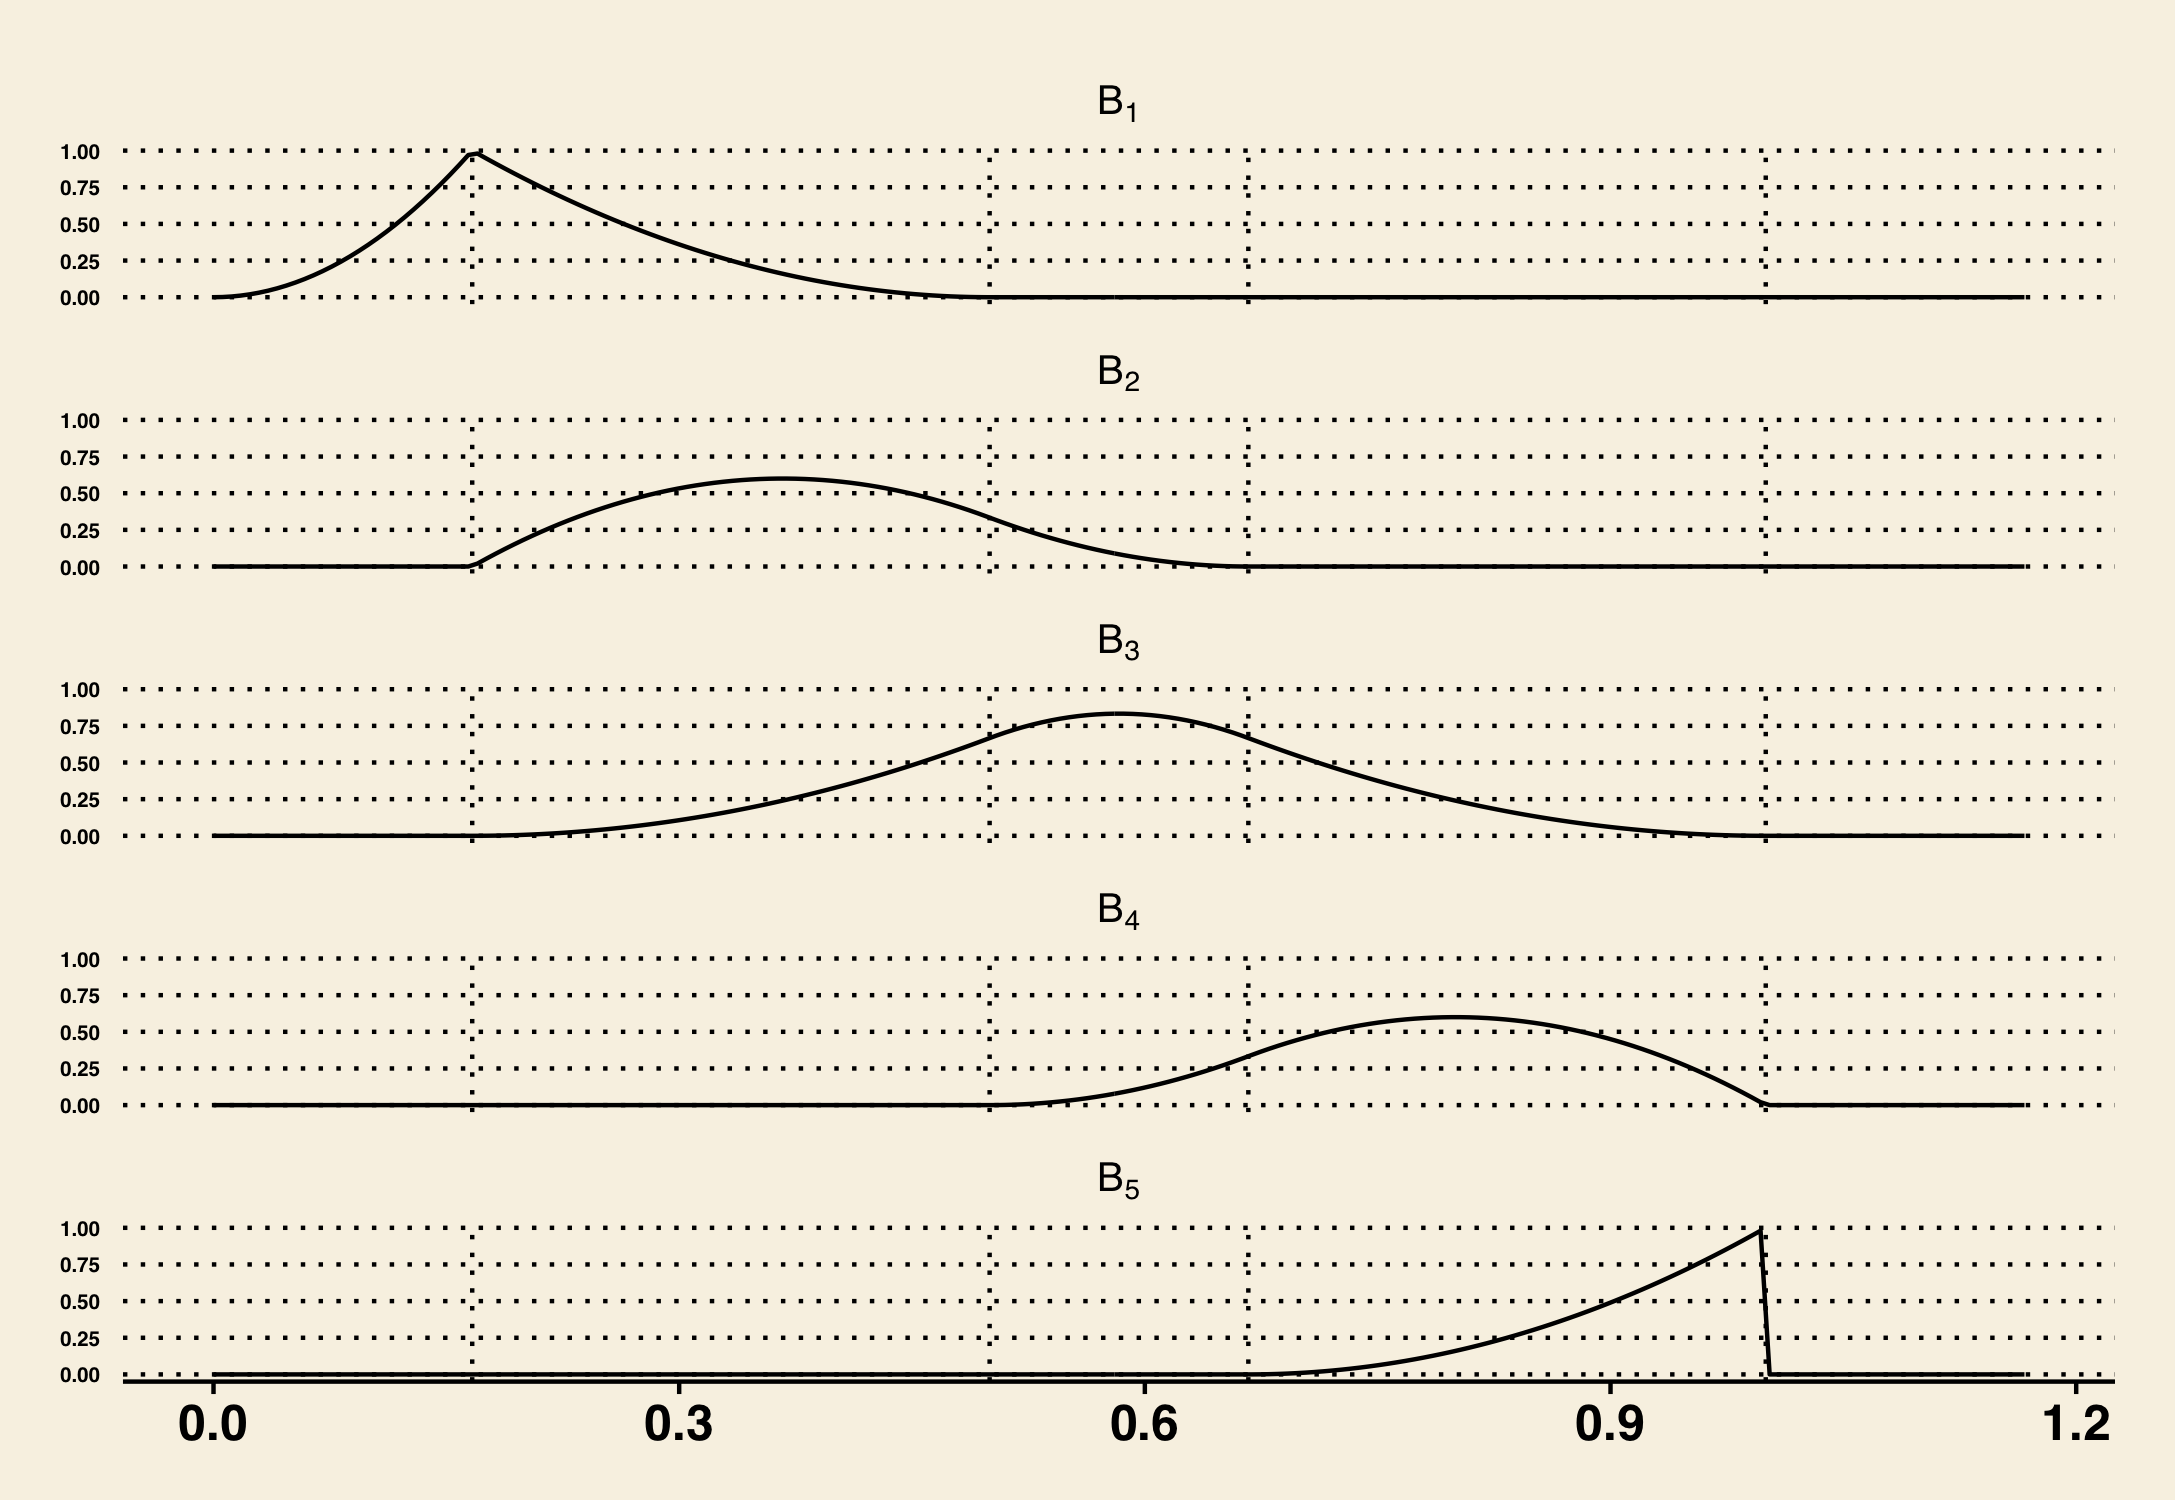
\includegraphics[width=7in, height=5in]{deboor_parabolic_bsplines.png}
  \caption{Parabolic B-splines corresponding to knot sequence $\{0,1,1,3,4,6,6,6\}$, illustrating the connection between knot multiplicity and smoothness.}\label{fig:deboor_bspline_basis}
\end{center}
\end{figure}
\end{example}


\begin{definition} \label{B_representation_definition}
The \emph{B-representation of } $f \in \PP_{k,\xi,\nu}$ consists of 
\begin{enumerate}
\item \label{eq:first_B_rep_piece} integers $k$ and $n$ specifying the order of $f$ as a pp function and the number of linear parameters, 
\[
n = kl - \sum_{i}\nu_i = \mbox{dim}\left(\PP_{k,\xi,\nu}\right),
\]
respectively. 
\item \label{eq:second_B_rep_piece}The knot vector $t = \left \{t_i \right\}$, $i=1,\dots, n+k$ with elements arranged in increasing order, constructed according to Theorem~\ref{curryschoenbergthm}, via $\xi$ and $\nu$.
\item \label{eq:third_B_rep_piece} The B-spline coefficients $\alpha=\left \{\alpha_i \right\}$, $i=1 ,\dots, n$ for the knot sequence, $t$.
\end{enumerate}
\end{definition}
\vspace{1pt}
Given \ref{eq:first_B_rep_piece}, \ref{eq:second_B_rep_piece}, and \ref{eq:third_B_rep_piece} in \ref{B_representation_definition}, the function value at $x\in \left[t_k, t_{n+1}\right]$ is given by 
\begin{equation*}
f\left(x\right) = \sum_{i=1}^n \alpha_i B_i\left(x\right),
\end{equation*}
and in particular, by \ref{eq:BS_property_1}, for $x\in \left[t_j, t_{j+1} \right]$,
\[
f\left(x\right) = \sum_{i=j}^{j+k-1} \alpha_i B_i\left(x\right).
\]





\section{Single-regressor varying coefficient models via B-spline basis expansions}

Hastie and Tibshirani were the first to introduce the varying coefficient model, which supplies a modeling approach which permits interpolation of regressors and response variables which varying according to an \emph{indexing variable} at values of this indexing variable where there is either missing data of only a single observation and slope estimation is not feasible. In the section that follows, we will discuss the approach to smoothing the coefficient vector (and \emph{not} the regressor, $x\left(t\right)$) first, for mechanical demonstration of parameterization and estimation of the coefficient function via B-spline basis expansion, at a predetermined set of values of an indexing variable, $t$ (knots), then following the approach of Eilers and Marx by assuming that the number and position of the knots are unknown and using penalized B-splines, or P-splines. 

Consider data of the form 
\[
\left(x_i, y_i, t_i\right), \qquad i=1,\dots,m
\]
where $y_i$ is the response, $x_i$ is the single (univariate) regressor variable, and $t_i$ is an indexing variable. We first consider a simple situation as an introductory warmup for demonstrating the mechanics of the varying coefficient model. Suppose we wish to fit a scatterplot smoother to the points $\left(t_i, y_i\right)$ using a B-spline basis expansion. Assume that we can model 

\begin{equation} \label{eq:varying_intercept_only_model}
y\left(t\right) = f\left(t\right) + \epsilon\left(t \right)
\end{equation}

where $\epsilon$ is a zero-mean error process.  Modeling the mean function as a $q^{th}$-order B-spline, we can rewrite \ref{eq:varying_intercept_only_model} as

\begin{equation} \label{eq:varying_intercept_only_model_bspline}
y\left(t\right) = \sum_{j=1}^{K} \alpha_j B_j\left(t\right) + \epsilon\left(t \right)
\end{equation}

Assume we use $K$ of basis functions in our expansion of $f$. Let $y= \left(y_1,\dots,y_m\right)^T$, and let $B$ denote the $m \times K$ design matrix with $i-j^{th}$ element given by the $j^{th}$ order-$q$ B-spline evaluated at the $i^{th}$ value of $t$: 

\[
b_{ij} = B_j\left(t_i\right),
\]
$i=1,\dots,m$, $j=1,\dots,K$. Then in matrix notation, we may write the mean vector

\[
\mu = E\left[y\right] = B\alpha
\]
\noindent
where $\alpha$ is the vector of $K$ unknown basis coefficients. We take $\hat{\alpha}$ to be the minimizer of 

\begin{align}
S &= \sum_{i=1}^m \left(y_i - \sum_{j=1}^{K} \alpha_j B_j\left(t_i\right) \right)^2 \nonumber\\
&=\vert y - B\alpha \vert^2 \label{eq:S_varying_intercept_model}
\end{align}


\[
B^TB\alpha = B^Ty
\]
which has explicit solution
\[
\hat{\alpha} = \left(B^T B\right)^{-1}B^Ty
\]

Given $\hat{\alpha}$, one may estimate the response at any new value of $t$, say $t^*$, by 
\[
\hat{y}\left(t^*\right) = \sum_{j=1}^{K} \hat{\alpha_j}B_j\left(t^*\right).
\]

\subsection{B-spline estimators for varying coefficient models with fixed knots}

To extend the varying intercept model \ref{eq:varying_intercept_only_model} to accommodate for controlling for another regressor, it is natural to consider the varying coefficient model; the single regressor varying-coefficient (VC) model extends the classical linear model by allowing the slope coefficient to vary smoothly in the dimension of the indexing variable, $t$.  The single-index varying coefficient model assumes that the mean response is of the form

\begin{equation} \label{eq:simplest_VC_model_mean}
E\left[ Y\left(t\right) \right] = \beta_0\left(t\right) + \beta_1\left(t\right)x\left(t\right)
\end{equation}

where $\beta_0\left(t\right)$ is the smooth varying intercept function and $\beta_1\left(t\right)$ is the smooth slope function of interest. This model generalizes the well known simple linear regression model 
\[
E\left[Y\left(t\right)\right] = \beta_0 + \beta_1 x\left(t\right)
\]
by trading the static regression coefficients for smooth coefficient functions which are assumed to varying across an indexing variable, $t$. This allows for the regressor variable to having modified effect, depending on the value of $t$. Using a set of predetermined knots along the $t$ axis, the VC model can be fit in a fashion similar to that required for fitting model \ref{eq:varying_intercept_only_model}, requiring only minor adjustments to the design matrix. In matrix notation as described in \ref{eq:S_varying_intercept_model}, the mean vector may be written

\begin{equation} \label{eq:VC_mean_matrix}
\mu = B\alpha_0 + diag\left\{x\left(t\right) \right\}B\alpha_1
\end{equation} 
\noindent
where $diag\left\{x\left(t\right) \right\}$ is the $m \times m$ diagonal matrix of regressor measurements which ensures that the varying coefficients are appropriately weighted according to the correct value of $x$ by aligning the regressor function with the corresponding slope value. Letting $U = diag\left\{x\left(t\right) \right\}B$, \ref{eq:VC_mean_matrix} becomes

\begin{align}
\mu &= \left[ B | U \right] \left(\alpha_0^T,\alpha_1^T\right)^T \\
&\equiv Q\alpha
\end{align} 

where $\alpha$ is the augmented vector of basis coefficients. Here, the same basis is used for smoothing both the varying intercept as well as the varying slope function; this is feasible because both components varying along the same indexing variable. One can relax this structure and allow each additive term to varying according to its own indexing variable. This, of course, requires a separate B-spline basis for each component. Again using least squares techniques as with the varying intercept-only model, we take $\hat{\alpha}$ to minimize

\begin{equation} \label{eq:S_varying_intercept_slope_model}
S = \vert y-Q\alpha \vert ^2
\end{equation}
which has explicit solution

\[
\hat{\alpha} =\left(Q^T Q\right)^{-1} Q^Ty.
\]

It is of interest to notice that $Q$ is simply a row scaling of the original B-spline design matrix, $B$; thus, accommodating a varying slope function equates to the simple basis function regression setting with a modified basis, $UB$. Using the modified basis functions as covariates, estimation of model the varying coefficient model equates to a multiple regression problem. Each of the estimated smooth components are given by 
\[
\hat{\beta}_k\left(t \right)= B\hat{\alpha}_k, \qquad k=0,1
\]
\noindent
and the estimate of the smooth mean function is obtained via 
\begin{align*}
\hat{\mu} &= Q\hat{\alpha}\\
&= Hy
\end{align*}
where $H = Q\left(Q^T Q\right)^{-1} Q^T$ is the ``hat'' matrix. This will be discussed in further detail in later sections on smoothing parameter selection and model tuning.





%%==============================================================================================================================================
%%==============================================================================================================================================
%%==============================================================================================================================================





\section{P-spline estimators for regularized estimation of fitted curves}

The mechanics in the previous section rely on apriori knowledge of the number and locations of the knots $\left\{t_j\right\}$, $j=1,\dots,K$. In practice this information is readily available, but has a considerable impact on the behaviour of the estimated coefficient functions, as the smoothness of a fitted curve can be controlled by the number of B-splines used in the basis expansion used to approximate the curve. Fewer knots (thus, fewer basis functions) lead to smoother fits. This choice presents a model selection problem, as too many knots lead to overfitting while too few knots lead to underfitting. Optimal knot placement has been closely examined, with some authors proposing automatic methods for optimizing the number and the positions of the knots (Friedman and Silverman, 1989; Kooperberg and Stone, 1991,1992). This is a difficult numerical problem requiring nonlinear optimization, and is still an open problem today. However, limiting the number of B-splines is not the only approach to controlling the complexity of the fitted function. 

As in chapter {\needsparaphrased{smoothing spline chapter}}, we can append a penalty on the coefficients of the basis functions to the goodness of fit measure, and by optimizing this augmented objective function, we can achieve as much smoothness in the fitted function as desired. \cite{o1986statistical} was the first to propose using a rich B-spline basis and applying a discrete penalty to the spline coefficients. 

 He proposed a penalty on the second derivative to restrict the flexibility of the fitted curve, similar to the penalty pioneered for smoothing splines by Reinsch (1967). This penalty has become the standard in much of the spline literature; see Eubank (1988), Wahba (1990) and Green and Silverman (1994). This measure of roughness of a curve is given by 
 
 \[
 J = \int_l^u \left[ f^{\prime \prime}\left(x\right)\right]^2\;dx
 \]
 \noindent
 where $l$ and $u$ are the bounds on the domain of $x$. Using the properties of B-splines, if $f\left(x\right) = \sum_{j} \beta_j B_j\left(x\right)$, one can derive a banded matrix $P$ such that 
 \[
 J = \beta^\prime P \beta
 \] 
 \noindent
 where $\beta = \left(\beta_1,\dots, \beta_n\right)$, and the $i$-$j^{th}$ element of $P$ is given by
 \[
 p_{ij} = \int_l^u B_i^{\prime \prime} \left( x \right)B_j^{\prime \prime} \left( x \right)\;dx.
 \]
 \noindent
 He then proposed minimizing
 \begin{eqnarray*}
 Q\left(\beta, \lambda \right) &=& \sum_{i=1}^m \left(y_i - \sum_{j} \beta_j B_j\left(x_i \right)\right)^2 + \lambda \int_l^u \left[ f^{\prime \prime}\left(x\right)\right]^2\;dx\\
 &=& \vert y - B\beta \vert  \vert^2 + \lambda\beta^\prime P \beta
 \end{eqnarray*}

The computation of $P$ is nontrivial and becomes very tedious when the third and fourth derivative are used as the roughness measure. \cite{wand2008semiparametric} extend O'Sullivan's work to higher order derivatives for general degree B-splines and derive an exact matrix algebraic expression for the penalty matrices. In the cubic case, the expression is a result of the application of Simpson's Rule applied to the inter-knot differences since each $B_i^{\prime \prime} B_j^{\prime \prime}$ is a piecewise quadratic function. The penalty may be written
 \[
 P = \left(B^{\prime \prime}\right)^\prime \textup{diag}\left(\omega \right) B^{\prime \prime}, 
 \]
 \noindent
 where $B^{\prime \prime}$ is the $3\left( n + 7 \right) \times \left( n + 4 \right)$ matrix with $i$-$j^{th}$ entry given by $B_j^{\prime \prime} \left(x_i^*\right)$, $x^*_i$ is the $i^{th}$ element of 
 
\[
\left( \phi_1,\frac{\phi_1+\phi_2}{2},\phi_2,\phi_2,\frac{\phi_2+\phi_3}{2},\phi_3,\dots,\phi_{n+7},\frac{\phi_{n+7}+\phi_{n+8}}{2},\phi_{n+8} \right),
\]
 \noindent
 and $\omega$ is the $3\left(n+7\right) \times 1$ vector given by
 
\begin{align*}
\omega &= \left( \frac{1}{6}\left(\Delta \phi \right)_1,\frac{4}{6}\left(\Delta \phi \right)_1, \frac{1}{6}\left(\Delta \phi \right)_1,\frac{1}{6}\left(\Delta \phi \right)_2, \frac{4}{6}\left(\Delta \phi \right)_2,  \right. \\
&\qquad   \left. {} \frac{1}{6}\left(\Delta \phi \right)_2 , \dots , \frac{1}{6}\left(\Delta \phi \right)_{n+7}, \frac{4}{6}\left(\Delta \phi \right)_{n+7}, \frac{1}{6}\left(\Delta \phi \right)_{n+7}  \right) \\
\end{align*}
\noindent
 where $\left(\Delta \phi \right)_j = \phi_{j+1}-\phi_j$. They generalize this to the case of any order penalty and present a table of formulas for constructing any arbitrary penalty matrix, $P$.
 
 %%==============================================================================================================================================
 
 \subsection{Difference penalties}
 
Imposing difference penalties on B-spline basis expansions generalizes and simplifies the approach outlined in the previous section in a way that permits application in any context where regression on B-splines is useful. Penalized B-splines, or \emph{P-splines}, are an alternative an approach to nonparametric smoothing which circumvent any complexity associated with constructing such penalty matrices by ommitting derivatives and integrals altogether. Instead, smoothness is imposed via a discrete penalty matrix based on finite difference formulas which is simple to compute. This approach achieves smoothness in fitted functions in two ways:

\begin{enumerate}
\item To avoid the difficulty of choosing the optimal set of knots, use a B-spline basis with a large number of equally spaced knots, purposefully overfitting the smooth coefficient vectors. 
\item Augment the goodness of fit measure with a difference penalty to prevent overfitting and accomodate a potentially ill-conditioned fitting procedure.
\end{enumerate}  
 
Using the properties of B-splines derived in {\needsparaphrased{B-spline section}}, it is relatively straightforward to show that the simplified penalty is nearly equivalent to the derivative-based penalty and that for second order differences, P-splines are very similar to O'Sullivan's approach. In some applications, it can be useful to use differences of a smaller or higher order in the penalty, and the P-spline framework makes the use of a penalty of any arbitrary order nearly seamless. 
 
Consider the varying intercept-only model defined in \ref{eq:varying_intercept_only_model} for the regression of $M$ data points $\left(t_i,y_i\right)$ on a set of $K$ B-splines, $\left\{B_j\right\}$.  By letting the number of knots, $K$, be relatively large, we allow more variation in fitted curve than the data reasonably justify. To make the result less flexible and avoid overfitting, O'Sullivan imposed a penalty on the second derivative of the fitted curve and appended this to the residual sum of squares, giving way to the objective function

\begin{equation} \label{eq:univariate_bspline_ridge_penalty}
\sum_{i=1}^m \left \{ y_i - \sum_{j=1}^K \beta_j B_j\left(t_i\right) \right \}^2 + \lambda \int_{t_{min}}^{t_{max}} \left\{  \sum_{j=1}^K \beta_j B^{\prime \prime}_j\left(t\right) \right\}^2 \; dt.
\end{equation}

The integral of the square of the second derivative of a fitted function has become common as a smoothness penalty since the seminal work on smoothing splines by Reinsch (1967), though it is useful to note that there is nothing particularly special about the second derivative. One could easily specify higher or lower order derivatives in smoothness penalties. In the context of smoothing splines, the first derivative leads to simple equations and a piecewise linear fit, while higher derivatives lead to systems of equations with a high bandwidth and a very smooth fit. 


Proposed for smoothing curves by \cite{whittaker1922new}, difference penalties have been utilized for nearly a century, with more recent applications  outlined in  \cite{eilers1991penalized}, \cite{eilers1991nonparametric}, and \cite{eilers1995indirect}. The finite difference penalty is easily introduced into regression equations, making it feasible to evaluate the impact of different orders of the differences on the fitted model. In some applications, it is useful to work with third and fourth order differences, since for high values of $\lambda$, the fitted curve approaches a parametric polynomial model. Detailed discussion on the effect of the smoothing parameter on fitted functions will follow. Let $D_d$ denote the matrix difference operator; that is, $D_d\beta = \Delta^d \beta$, where

 \begin{eqnarray*}
 \Delta \alpha_j &=& \alpha_j - \alpha_{j-1},\\
 \Delta^2 \alpha_j &=& \Delta\left(\Delta \alpha_j\right) = \alpha_j - 2\alpha_{j-1} + \alpha_{j-2},\\ 
 \end{eqnarray*}
\noindent 
and in general,
\begin{equation*}
\Delta^d \alpha_j = \Delta\left(\Delta^{d-1} \alpha_j \right)
\end{equation*}
The $\left(K - d\right) \times K$ differencing matrix $D_d$ is sparse for reasonably small values of $d$; for example, $D_1$ and $D_2$ for small dimensions are given by 
\[
D_1 = \begin{bmatrix} -1&1&0&0\\ 0&-1&1&0\\ 0&0&-1&1 \end{bmatrix}; \qquad D_2 = \begin{bmatrix} 1&-2&1&0 \\ 0&-&-2&1\end{bmatrix}
\]

\cite{eilers1996flexible} propose to base the penalty on (higher-order) finite differences of the coefficients of adjacent B-splines:

 \[
 \lambda\vert D_d\alpha\vert^2 = \lambda \alpha^\prime D^\prime_d D_d \alpha = \lambda \alpha^\prime P\alpha,
 \] 



Replacing O'Sullivan's penalty with the difference penalty, we can control the smoothness of the fitted mean function $\mu = \beta_0\left( t \right) = B\alpha$ by minimizing
\begin{equation*} 
S_\lambda = \vert y- B \alpha \vert^2 + \lambda\vert D_d\alpha \vert^2
\end{equation*}

This approach reduces the dimensionality of the problem to the number of B-splines, $K$ instead of the number of observations, $M$ , as with smoothing splines. The tuning parameter $\lambda$ permits continuous control over smoothness of the fit. We will demonstrate that the difference penalty is a good discrete approximation to the integrated square of the $k^{th}$ derivative, and with this penalty, moments of the data are conserved and polynomial regression models occur as limits for large values of $\lambda$. We will explore the connection between a penalty on second-order differences of the B-spline coefficients and O'Sullivan's choice of a penalty on the second derivative of the fitted function. However, the difference penalty can be handled mechanically for any order of the differences.
\cite{o1986statistical} used third-degree B-splines and the following penalty:

\begin{equation} \label{eq:osullivan_univariate_bspline_penalty}
h^2 P = \lambda \int_{t_{min}}^{t_{max}} \left\{ \sum_{j}  \alpha_j B_{j,3}^{\prime \prime} \left(t\right) \right\}^2\; dt
\end{equation}
\noindent
From the derivative properties of B-splines, it follows that
\begin{equation} \label{osullivan_univariate_bspline_penalty_via_deriv}
h^2 P = \lambda \int_{t_{min}}^{t_{max}}  \sum_{j} \sum_{k} \Delta^2 \alpha_j \Delta^2 \alpha_k B_{j,1}\left(t\right)B_{k,1}\left(t\right) dt 
\end{equation}
\noindent
Most of the cross products of $B_{j,1}(t)$ and $B_{k,1}(t)$ vanish since B-splines of degree 1 only overlap when $j$ is $k-1$, $k$, or $k+1$. Thus, we have that
\begin{align}
h^2 P = {} & \lambda \int_{t_{min}}^{t_{max}} \bigg[ \left\{ \sum_{j}  \Delta^2 \alpha_j  B_j\left(t,1\right)  \right\}^2  + 2 \sum_{j}\Delta^2 \alpha_j\Delta^2 \alpha_{j-1}B_j\left(t,1\right)B_{j-1}\left(t,1\right) \bigg] dt \nonumber \\ 
= {} & \lambda \bigg[ \sum_j \left( \Delta^2\alpha_j \right)^2 \int_{t_{min}}^{t_{max}} B_j^2\left(t,1\right)\;dt + 2 \sum_j \Delta^2 \alpha_j\Delta^2 \alpha_{j-1} \bigg]
\end{align}
\noindent
or
\begin{align}
h^2 P = \lambda \sum_j \left( \Delta^2\alpha_j \right)^2 \int_{t_{min}}^{t_{max}} B_{j,1}^2\left(t\right) dt {} & +  2\lambda \sum_j \Delta^2 \alpha_j \Delta^2 \alpha_{j-1}  \nonumber \\ 
{} &+\int_{t_{min}}^{t_{max}} B_{j,1}\left(t\right)B_{j-1,1}\left(t\right) dt
\end{align}
\noindent
which can be written as
\begin{equation} \label{eq:osullivan_penalty_decomp}
h^2 P = \lambda\left\{c_1 \sum_j\left( \Delta^2 \alpha_j\right)^2 + c_2 \sum_j\Delta^2 \alpha_j\Delta^2 \alpha_{j-1} \right\}
\end{equation}
\noindent
where, for given equidistant knots, $c_1$ and $c_2$ are constants given by
\begin{equation}
\begin{split}
c_1 & =   \int_{t_{min}}^{t_{max}} B_{j,1}^2\left(t\right) dt\\
c_2 & = \int_{t_{min}}^{t_{max}} B_{j,1}\left(t\right)B_{j-1,1}\left(t\right) dt
\end{split}
\end{equation}

O'Sullivan's ridge-like B-spline penalty in Equation~\ref{eq:osullivan_univariate_bspline_penalty} can be written as a linear combination of a difference penalty (\ref{eq:univariate_pspline_diff_penalty}) and the sum of the cross products of neighboring second differences. The second term in Equation~\ref{eq:osullivan_penalty_decomp} leads to a complex objective function when minimizing the penalized likelihood, where seven adjacent spline coefficients occur, as opposed to five if only the first term in Equation~\ref{eq:osullivan_penalty_decomp} is used in the penalty. The additional complexity is due to overlapping B-splines, which quickly increases when using higher order differences and higher order B-splines. The use of a difference penalty allows us to sidestep the difficulty of constructing a procedure for incorporating the penalty in the likelihood equations. 

Define $\hat{\alpha} = \left(\hat{\alpha}_1, \hat{\alpha}_2, \dots, \hat{\alpha}_K \right)$ to be the minimizer of $S_\lambda$:

\begin{equation*}  
S_\lambda = \sum_{i=1}^m \left\{ y_i - \sum_{j=1}^K \alpha_j B_j\left(t_i\right) \right\}^2 + \lambda \sum_{j=d+1}^K \left( \Delta^d\alpha_j \right)^2
\end{equation*}
\noindent
In vector notation, this may be written

\begin{align}
\begin{split}
S_\lambda &= \vert y- B\alpha  \vert^2  + \lambda \vert D_d \alpha\vert^2 \\
&=  \left( y- B\alpha  \right)^T \left( y-B \alpha\right) + \lambda \alpha^T P \alpha
\end{split} \label{eq:S_pen_varying_intercept_model}
\end{align}
\noindent
where 
\[
P = D_d^T D_d
\]
\noindent
and the elements of $B$ are given by $b_{ij} = B_j\left(t_i\right)$, as defined in \ref{eq:S_varying_intercept_model}. Taking derivatives on both sides of \ref{eq:S_pen_varying_intercept_model} with respect to $\alpha$ gives

\begin{align}
\frac{\partial}{\partial \alpha}S_\lambda ={} & \frac{\partial}{\partial \alpha}\left(\alpha^TB^TB \alpha -2y^T B^T\alpha+\lambda \alpha^T D_k^T D_k \alpha  \right) \nonumber \\
= {} & 2B^TB \alpha - 2B^T y + 2\lambda D_d^TD_d\alpha \nonumber\\
= {} & \left(B^T B +  \lambda D_d^TD_d\right)\alpha - B^T y \label{eq:dSlambda_dAlpha}
\end{align} 
\noindent

and setting equal to zero yields normal equations:
\begin{equation}\label{eq:S_lambda_normal_eq}
B^T y = \left(B^T B +  \lambda D_d^TD_k\right)\alpha,
\end{equation}
which has explicit solution
\[
\hat{\alpha} = \left(B^T B +  \lambda D_d^TD_d\right)^{-1}B^T y
\]
\noindent
The effective hat matrix is now
\[
H_\lambda - B\left(B^T B +  \lambda D_k^TD_k\right)^{-1}B^T 
\]

When $\lambda = 0$, we have the standard normal equations of linear regression with a B-spline basis, and with $k = 0$ \ref{eq:S_lambda_normal_eq} corresponds to the normal equations under the ridge regression penalty. When $\lambda > 0$, the penalty only influences the main diagonal and $k$ sub-diagonals of the system of equations. The compact support and limited overlap of the B-spline basis functions gives this system a banded structure, though exploiting this structure is of little utility since the number of equations is equal to the number of splines, which is generally moderate by design. 



\subsubsection{P-splines for single-index VC models}

The derivations in the previous section requiring little adjustment for accommodating a regressor and its corresponding varying slope function, as defined in Equation~\ref{eq:simplest_VC_model_mean} with $\mu\left(t\right) =  Q\alpha$, where 
\[
Q = \left[B | diag\left\{x\left(t\right) \right\}B \right]
\]
but now $B$ holds a rich B-spline basis with equally-spaced knots. If one wishes to allow for differing degrees of smoothing for each of the varying intercept term and the slope function, the P-spline objective function \ref{eq:S_pen_varying_intercept_model} must be further modified to accommodate multiple tuning parameters, $\lambda_i$, $i=0,1$. The objective function then becomes
\begin{align} 
\begin{split}
S^*_\lambda &= \vert y- Q\alpha  \vert^2  + \lambda_0 \vert D_{d_0} \alpha_0 \vert^2 + \lambda_1 \vert D_{d_1} \alpha_1 \vert^2\\
	&= \vert y- Q\alpha  \vert^2  + \vert \alpha^T P \alpha \vert^2
\end{split} \label{eq:S_pen_star}
\end{align}

where the penalty has form $P = \mbox{block diag}\left(\lambda_0 D_{d_0}^TD_{d_0}, \lambda_1 D_{d_1}^TD_{d_1} \right)$. The minimizer of \ref{eq:S_pen_star} is given by
\[
\hat{\alpha} = \left(Q^T Q +  P\right)^{-1}Q^T y.
\]

The block diagonal structure of the penalty separates the penalization of each individual smooth component. The estimated mean function is then given by 
\[
\hat{\mu} = Q \hat{\alpha} = H y
\] 
where
\begin{equation} \label{eq:simplest_VC_model_hat_matrix}
H = Q\left(Q^T Q +  P\right)^{-1}Q^T.
\end{equation}

{\needsparaphrased{[Figure~\ref{fig:PS_VCM_section_figure_1} Need to explain figure 3 here. ]} }

\begin{figure}[H]
   \graphicspath{{img/}}
   \centering
  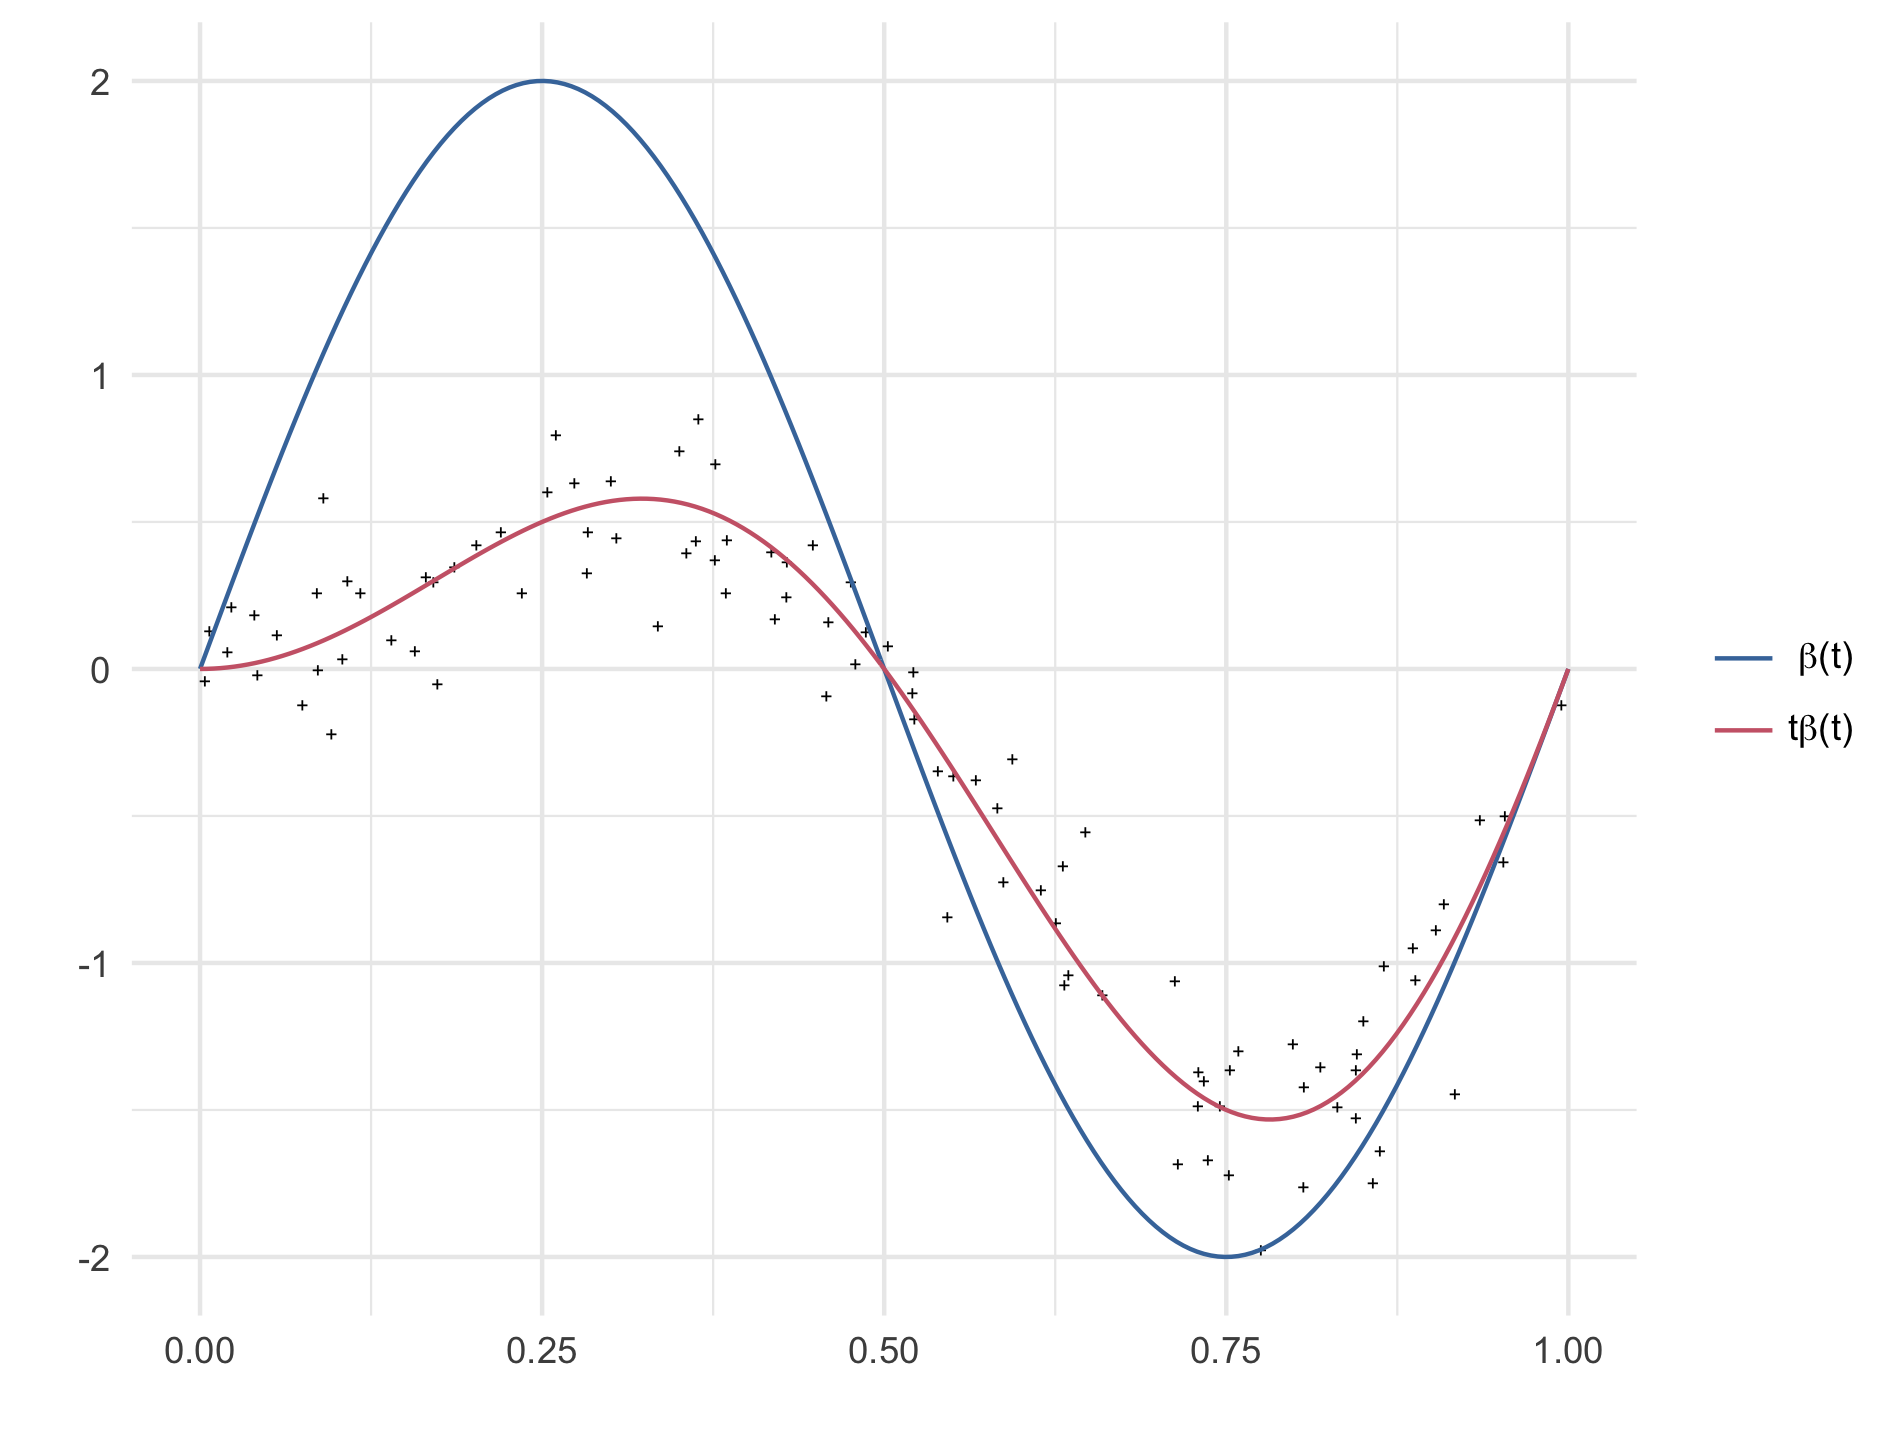
\includegraphics[scale=0.25]{PS_VCM_section_figure_1.png}
\caption{\textit{100 simulated data points where} $y\left(t\right) = t \beta\left( t \right) + 0.2\epsilon\left(t\right)$ \textit{where} $\epsilon$ \textit{is a white noise process with unit variance, and} $\beta\left(t\right) = 2\sin\left(2\pi t\right)$.}
\label{fig:PS_VCM_section_figure_1}
\end{figure}

\begin{figure}[H]
 \begin{subfigure}{.48\textwidth}
  \centering
   \graphicspath{{img/}}
 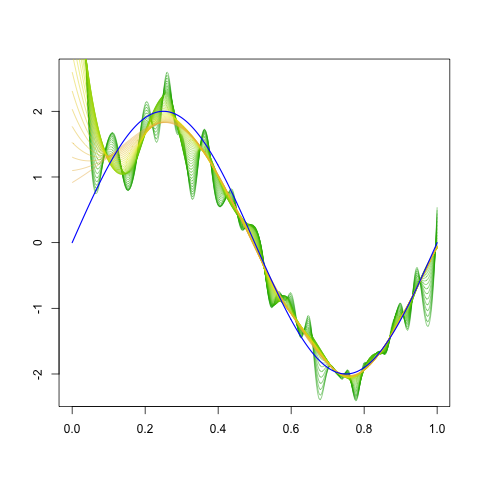
\includegraphics[scale=0.5]{PS_VCM_section_figure_2.png}
 \caption{$\hat{\beta}\left(t\right)$}
 \end{subfigure}
 \begin{subfigure}{.48\textwidth}
  \centering
   \graphicspath{{img/}}
  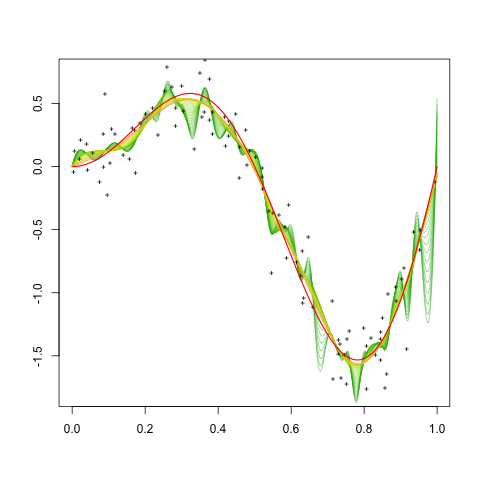
\includegraphics[scale=0.5]{PS_VCM_section_figure_3.png}
 \caption{$\hat{\mu}\left(t\right) = t \hat{\beta}\left(t\right)$}
\label{fig:PS_VCM_section_figure_2}
 \end{subfigure}
 \caption{\textit{Estimated coefficient function} $\hat{\beta}\left(t\right)$ \textit{and mean curve} $\hat{\mu}\left(t\right) = t \sin(2 \pi t)$ \textit{using a 80 B-splines basis functions of order 5 and a difference penalty of order} $k=3$.}
\end{figure}




The properties discussed in Section~\ref{BS_properties_continued} allude to how controlling the coefficients of a spline $f \in \mathscr{S}_{k,t}$ influences the shape of the overall function. Specifically, the form of the $j^{th}$ derivative provides an avenue of understanding how the differenced B-spline coefficient sequence is related to the volatility of the function on a given interval of its domain. The following figure visually explore the impact of the squared distance on adjacent basis coefficients on the function; a useful way of examining at P-splines is to consider the coefficients as the skeleton of the function, then draping the B-splines over them to put the flesh over the bones. A smoother sequence of coefficients leads to a smoother curve, which is clearly illustrated in Figure~\ref{fig:second_ord_PS_pen_SML_lambda}. As long as the coefficient sequence is smooth, the number of basis functions (and coefficients) is unimportant. The penalty ensures the smoothness of the skeleton.

\begin{figure}[H]
\begin{subfigure}{.5\textwidth}
  \centering
   \graphicspath{{img/}}
  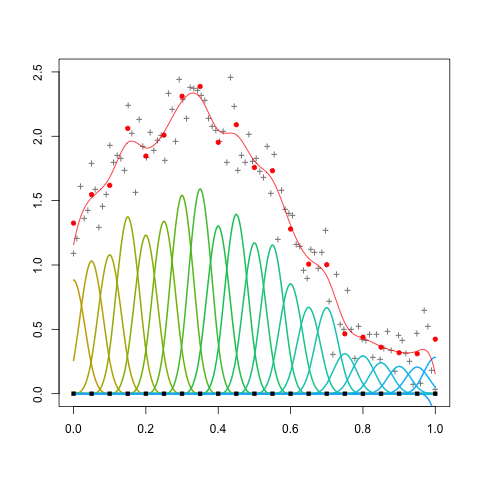
\includegraphics[scale=0.5]{pspline_pord2_xsmall_lambda.png}
  \label{fig:pspline_small_lambda}
\end{subfigure}
\begin{subfigure}{.5\textwidth}
  \centering
   \graphicspath{{img/}}
  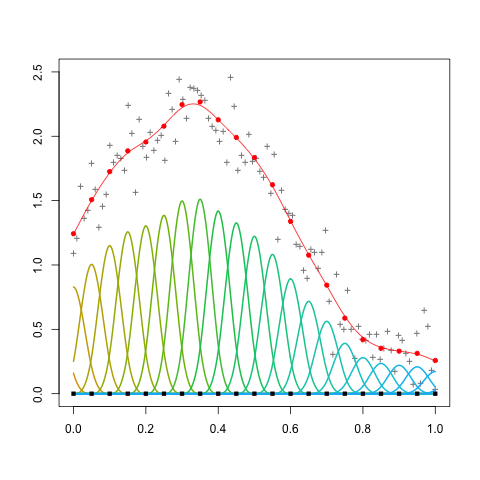
\includegraphics[scale=0.5]{pspline_pord2_small_lambda.png}
  \label{fig:pspline_small_lambda}
\end{subfigure}
\begin{subfigure}{.5\textwidth}
  \centering
   \graphicspath{{img/}}
  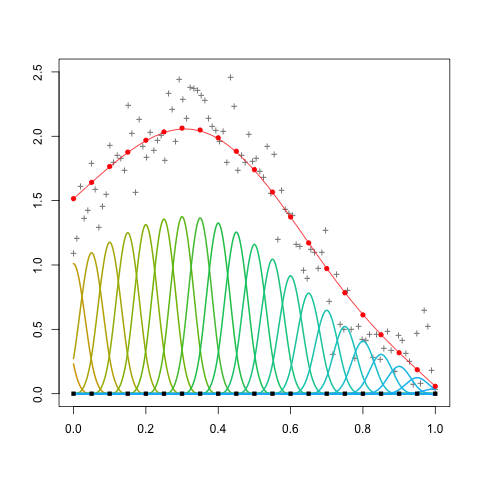
\includegraphics[scale=0.5]{pspline_pord2_medium_lambda.png}
  \label{fig:pspline_small_lambda}
\end{subfigure}
\begin{subfigure}{.5\textwidth}
  \centering
   \graphicspath{{img/}}
  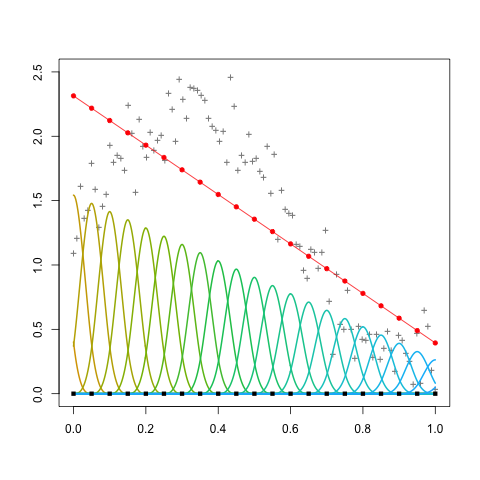
\includegraphics[scale=0.5]{pspline_pord2_large_lambda.png}
  \label{fig:pspline_small_lambda}
\end{subfigure}
\caption{\textit{Illustration of the impact of the second order difference penalty. The number of B-splines used is the same in each plot, with the value of the penalty parameter increasing from left to right and top to bottom across each plot. The fitted curve in the upper left plot is the most ``wiggly'' of any of the fits, as the penalty plays the weakest roll in the fitted coefficients there. The red circles are the values of each of the B-spline coefficients; as the penalty increases, they form as smoother sequence as we move across the four plots, which results in a smoother fitted function. As the penalty parameter approaches infinity, the fit approaches a linear function as shown in the bottom right plot.}}
\label{fig:second_ord_PS_pen_SML_lambda}
\end{figure}

The number of B-splines can be much larger than the number of observations because penalty ensures that the fitting procedure well-conditioned. One could literally use a thousand splines to fit ten observations without problems. Figure~\ref{fig:overcomplete_basis_pspline} illustrates this utility of the penalty for simulated data. There are $m=10$ observations and $40 + 3$ cubic B-splines. This property of P-splines cannot be overly appreciated, as it allows us to completely circumvent the nontrivial task of the optimal selection of knot placement. But one simply cannot have too many B-splines. Unless computational constraints are of concern, which is possible with large models, it is prudent to use even more. Figure~\ref{fig:PS_penalty_section_figure_3} shows how the fitted function changes as the tuning parameter $\lambda$ is varied in the presence of sparsely sampled data. 

\begin{figure}[H]   \label{fig:overcomplete_basis_pspline}
  \centering
   \graphicspath{{img/}}
  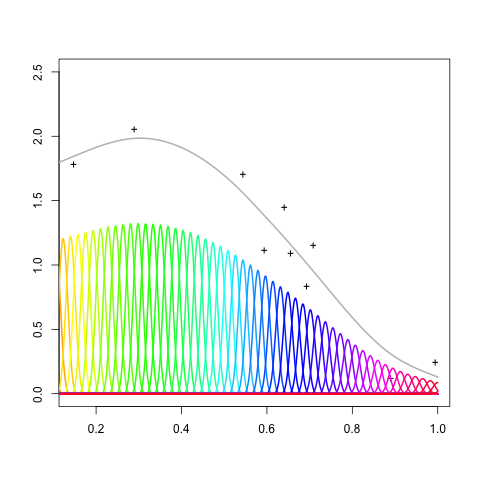
\includegraphics[scale=0.75]{pspline_10obs_60_basis_functions.png}
  \caption{P-spline smoothing of 10 observations using 60 B-spline basis functions.}
\end{figure}

\begin{figure}[H] \label{fig:PS_penalty_section_figure_3}
\centering
 \graphicspath{{img/}}
  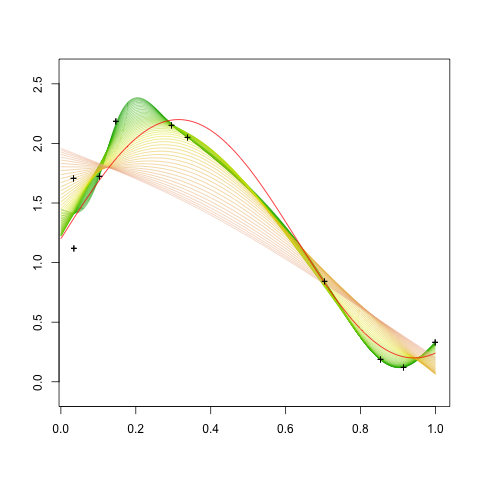
\includegraphics[width=4in, height=4in]{PS_penalty_section_figure_3.png}

  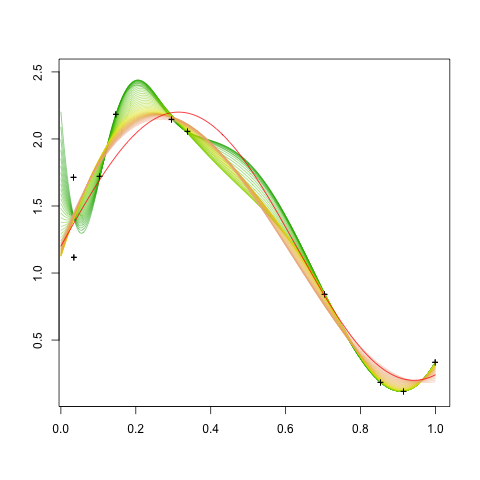
\includegraphics[width=4in, height=4in]{PS_penalty_section_figure_4.png}
 \caption{Fitted mean curves using a second (top) and third (bottom) order difference penalty for simulated data, sparsely sampled along the indexing variable: $y\left(t\right) = 1.2 + \sin\left(5t\right) + 0.2\epsilon_t$, where $\epsilon_t \stackrel{i.i.d.}{\sim}\textup{N}\left(0,1\right)$. A total of 10 data points were fit using a basis of 60 B-splines of degree $k=3$.}
\end{figure}

%%====================================================================================

\subsection{Properties of P-splines}

P-splines enjoy many advantageous properties, many due in part to the inherited properties of the B-spline basis functions on which a generous portion of their foundation is constructed. 

\begin{enumerate} \label{eq:PS_properties}
\item \begin{description}\item[Boundary effects]
 P-splines show no boundary effects, as many types of kernel smoothers do. By this, we mean the spreading of a fitted curve or density outside of the (physical) domain of the data, generally accompanied by bending toward zero.
\end{description}
\item \begin{description}\item[P-splines fit polynomial data exactly.] 
P-splines can fit polynomial data exactly. Given data $\left(t_i,y_i\right)$, if the $y_i$ are a polynomial in $t$ of degree $k$, then B-splines of degree $k$ or higher will fit the data exactly. 
\begin{proof}
This statement is equivalent to the claim that given $\xi = \left\{ \xi_i \right\}$, $i=1,\dots,l+1$, and $g$ such that $y\left(t\right) = g\left(t\right)$, we can find an $f \in \PP_{k,\xi} \bigcap \mathscr{C}^{\left(k-2\right)}$ which agrees with $g$ at the points $\tau_1 < \dots < \tau_n$  with $\tau_i \in \left[\xi_1,\xi_{l+1}\right]$ for all $i$, where
\[
n=k+l-1
\]
The solution, $f$ is constructed as follows: generate the knot sequence $t = \left\{t_i\right\}$ as per the recipe in Theorem~\ref{curryschoenbergthm}:
\begin{align*}
t_1 &= t_2 = \dots = t_k = \xi_1 & \\
t_{k+i} &= \xi_{i+1}, & i=1,\dots,l-1\\
t_{n+1} &= t_{n+2} = \dots = t_{n+k} = \xi_{l+1} & 
\end{align*}

Let $\left\{ B_{ik} \right\}$, $i=1,\dots,n$ be the corresponding sequence of B-splines of order $k$, which are a basis for $\PP_{k,\xi} \bigcap \mathscr{C}^{\left(k-2\right)}$ by Theorem~\ref{curryschoenbergthm}. Here, $\PP_{k,\xi} \bigcap \mathscr{C}^{\left(k-2\right)}$ denotes the space of pp functions with breakpoints $\xi$ having two continuous (global) derivatives. Then, \cite{schoenberg1953polya} have shown that there exists exactly one $f \in \PP_{k,\xi} \bigcap \mathscr{C}^{\left(k-2\right)}$ agreeing with $g$ at $\tau_1,\dots, \tau_n$ if and only if 
\[
B_{ik}\left(\tau_i\right) \ne 0, \qquad \qquad i=1,\dots,n.
\]
This $f$ has a unique expansion of the form
\[
f = \sum_{i=1}^n a_i B_{ik}
\] 
for coefficients $a_i,\dots, a_n$, which are the solution to the linear system
\[
\sum_{j=1}^n a_jB_{jk}\left(\tau_i\right) = g\left(\tau_i\right), \qquad \qquad i=1,\dots,n.
\]
This system has a banded matrix of coefficients since $B_{jk}\left(\tau_i\right) \ne 0$ if and only if $\tau_i \in \left[t_j,t_{j+k}\right]$. So if $B_{jk}\left(\tau_i\right) \ne 0$ and thus $\tau_i \in \left(t_j,t_{j+k}\right)$, then there are at most $k$ of the $j$ indices such that $B_{jk}\left(\tau_i\right)$ is nonzero. And further, each of these indices $j$ must be such that 
\[
\left(t_i,t_{i+k}\right) \bigcap \left(t_j,t_{j+k}\right) \ne \emptyset,
\]
or such that $\vert i-j \vert < k$. At worst, the system corresponds to a banded matrix with $k-1$ lower and $k-1$ upper diagonals. 
\end{proof}
The same is true for P-splines if the order of the penalty is $k+1$ or higher, irrespective of the value of $\lambda$. Consider imposing a first-order difference penalty and a fit to data $y$ that is constant - a polynomial of degree 0. Since 
\[
\sum_{j=1}^n \hat{\alpha}_j B_j\left( x_i \right) = c, 
\]
\noindent
we have that
\[
\sum_{j=1}^n \hat{\alpha}_j B^\prime_j\left( x \right) = 0, 
\]
\noindent
for all $x$. From the relationship between differences and derivatives in \ref{eq:more_BS_properties} \ref{eq:BS_deriv_property}, 

\[
0 = \sum_{j=1}^n B^\prime_{j,k}\left(x\right) = \sum_{j=1}^n \Delta\alpha_{j+1} B_{j,k-1}\left( x \right), 
\]
\noindent
so that we must have $\Delta \alpha_j = 0$ for all $j$, and 
\[
\sum_{j=2}^n \Delta \alpha_j = 0.
\]

This shows that the penalty has no impact on the basis coefficients, and the resulting fit is identical to that when using unpenalized B-splines. Using induction, one can show that this is also true when the relationship between $x$ and $y$ is linear and a second order difference penalty is used, and for any values of the polynomial order and order of the difference penalty.\end{description}
\item \begin{description}\item[Null models under difference penalties] \label{eq:PS_property_3}
The limiting P-spline fit approaches a polynomial under strongly enforced smoothing. As $\lambda \rightarrow \infty$, under a difference penalty of order $d$, the fitted function will approach a polynomial of degree $d-1$ as long as the degree of the B-splines is greater than or equal to $k$. To see this, we again need to use the relationship between the differenced coefficient sequence and the derivative of a B-spline as described in \ref{eq:more_BS_properties} \ref{eq:BS_deriv_property}. Consider using the second-order difference penalty; when $\lambda$ is large, the penalty dominates the P-spline objective function defined in \ref{eq:S_pen_varying_intercept_model}, so that the minimizer $\alpha$ must be such that $\sum_{j=3}^n\left(\Delta^2\alpha_j\right)^2$ is close to zero. Consequently, each of the individual second differences must also be nearly zero, and thus the second derivative of the fitted function must be close to zero over the entire domain.
\end{description}
\item \begin{description}\item[The limiting behaviour of $H_\lambda$] The trace of the hat matrix, 
\[
H_\lambda = B\left(B^TB + \lambda D_k^TD_k\right)^{-1}B^Ty
\] 
(or for $H$ defined for the addition of a varying slope component as in \ref{eq:simplest_VC_model_hat_matrix}) approaches $k$, the order of the differencing operator, as $\lambda$ increases. We index $H$ with the smoothing parameter to indicate that the elements of $H$ are a function of $\lambda$. Let
\begin{equation}
Q_B = B^T B \qquad \mbox{and} \qquad Q_\lambda = \lambda D^T D.
\end{equation}
Then using properties of the matrix trace, we can write
\begin{align}
\begin{split}
\mbox{tr}\left(H_\lambda \right) &= \mbox{tr}\bigg[ \left(Q_B + Q_\lambda \right)^{-1}Q_B \bigg]\\
&=\mbox{tr}\bigg[ Q_B^{1/2}\left(Q_B + Q_\lambda \right)^{-1}Q_B^{1/2} \bigg] \\
&=\mbox{tr}\bigg[\left(I + Q_B^{-{1/2}}Q_\lambda Q_B^{-{1/2}} \right)^{-1} \bigg]
\end{split}
\end{align}
Define $L \equiv Q_B^{-{1/2}}Q_\lambda Q_B^{-{1/2}}$. Then
\begin{equation}
\mbox{tr}\left(H_\lambda \right) = \mbox{tr}\bigg[\left(I + \lambda L \right)^{-1} \bigg] = \sum_{j=1}^n \frac{1}{1 + \lambda \gamma_j}
\end{equation}
 where $\gamma_j$, $j=1,\dots,n$ are the eigenvalues of $L$. $Q_\lambda$ has exactly $k$ eigenvalues equal to zero, hence $L$ has $k$ zero eigenvalues. For large $\lambda$, only the $k$ terms with $\gamma_j=0$ contribute to the sum which gives the trace of $H$, so that
 \[
\lim_{\lambda \rightarrow \infty  } \mbox{tr}\left(H\right) = k.
 \]
\end{description}
\end{enumerate}

The previous derivations hold regardless of whether we are fitting the varying intercept-only model, with $\mu\left( t\right) = \beta_0\left(t\right)$ or accommodating a varying slope for a regressor by specifying $\mu\left( t\right) = \beta_0\left(t\right) + \beta_1\left(t\right)x\left(t\right)$. The inspection of the hat matrix $H$ is a prelude to the following section, where we will discuss how to use the properties of $H$ to tune the smoothing parameter for optimal model selection. We will later show that extension of these results can be extended in a rather straightforward manner to the case that is of our particular interest: when the smooth slope function is a two-dimensional surface rather than a curve.

\begin{figure}[H]
\begin{subfigure}{.5\textwidth}
  \centering
   \graphicspath{{img/}}
  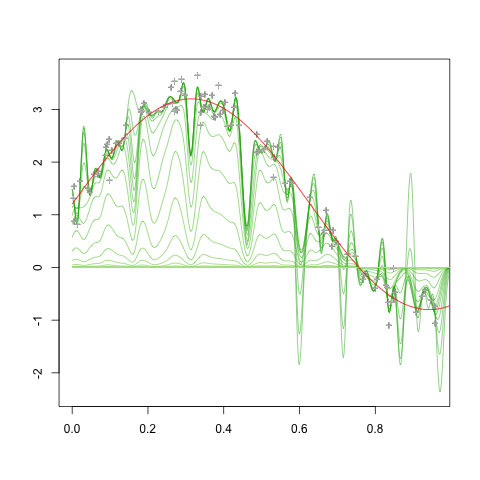
\includegraphics[scale=0.5]{PS_penalty_section_figure_6_order_0.png}
  %\label{fig:pspline_small_lambda}
\caption{$d=0$ }
\end{subfigure}
\begin{subfigure}{.5\textwidth}
  \centering
   \graphicspath{{img/}}
  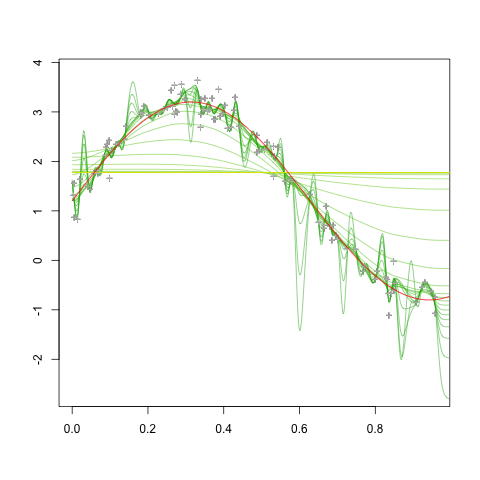
\includegraphics[scale=0.5]{PS_penalty_section_figure_6_order_1.png}
 % \label{fig:pspline_small_lambda}
\caption{$d=1$}
\end{subfigure}
\begin{subfigure}{.5\textwidth}
  \centering
   \graphicspath{{img/}}
  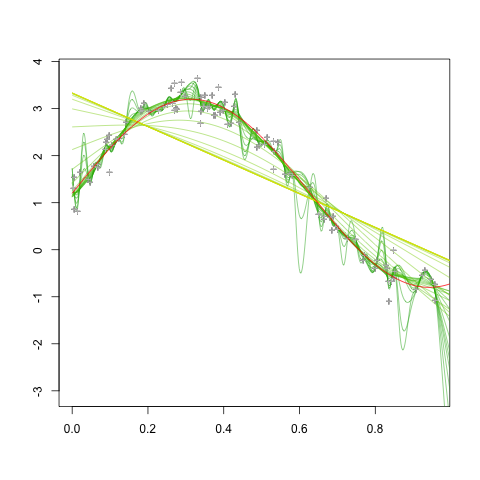
\includegraphics[scale=0.5]{PS_penalty_section_figure_6_order_2.png}
  %\label{fig:pspline_small_lambda}
\caption{$d=2$}
\end{subfigure}
\begin{subfigure}{.5\textwidth}
  \centering
   \graphicspath{{img/}}
  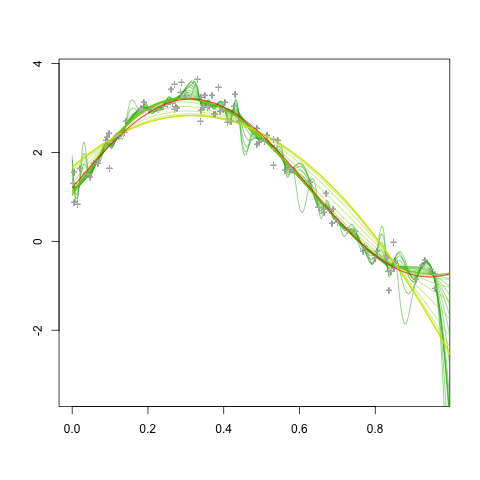
\includegraphics[scale=0.5]{PS_penalty_section_figure_6_order_3.png}
  %\label{fig:pspline_small_lambda}
\caption{$d=3$}
\end{subfigure}
\caption{\textit{Illustration of the impact of the order of the difference penalty. The number of B-splines used is the same in each plot, with the penalty parameter varying from across the same grid of values. The fitted curves in the upper left plot correspond to the difference penalty of order $0$, where $\vert D_0 \alpha \vert^2 = \sum_{i=1}^n \alpha_i^2$, analogous to ridge regression using the B-spline basis as regression covariates. The fitted curves approach polynomials of degree $d-1$ as $\lambda \rightarrow \infty$, as discussed in \ref{eq:PS_properties} \ref{eq:PS_property_3}.}}
\label{fig:PS_penalty_section_figure_6}
\end{figure}




\begin{figure}[h]
\centering
 \graphicspath{{img/}}
  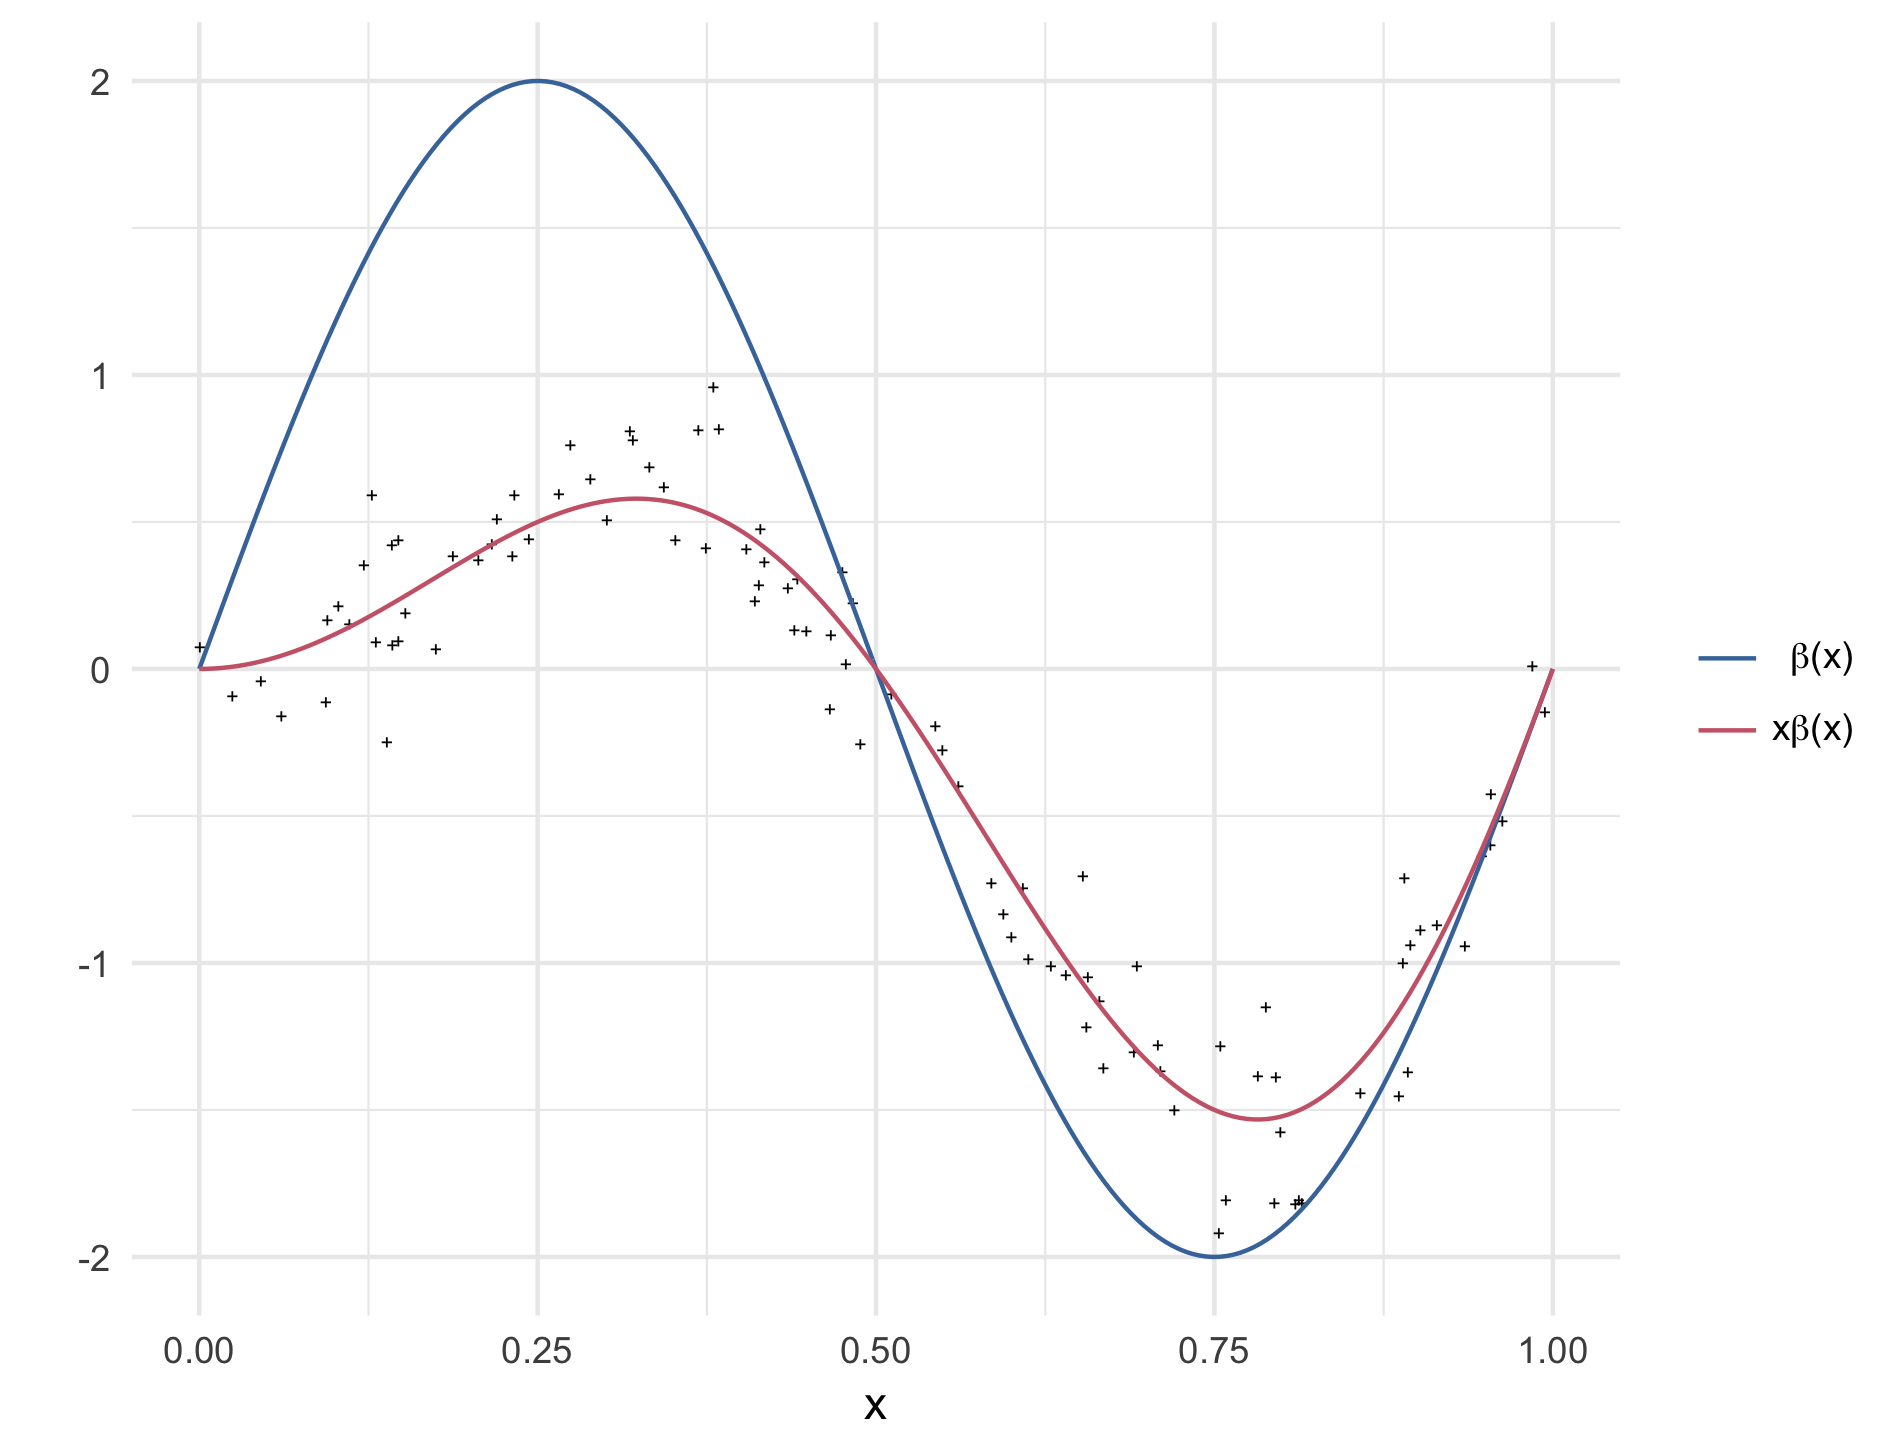
\includegraphics[width=4in, height=4in]{PS_penalty_section_figure_5.png}
 %\caption{Tensor product of two cubic B-splines}
\end{figure}




%\begin{equation}
%J\left(\phi^*\right) = 
%\end{equation}
%%%% Instead of using 2, could formulate this in terms of general k as well







%\begin{eqnarray}
%R_l\left(l,l^\prime\right) &=& \sum_{j=0}^k l^k {l^{\prime}}^k + \sum_{i=1}^{\vert \vert \mathcal{L}\vert \vert} T^*_{i,k}\left(l\right)T^*_{i,k}\left(l^\prime\right)
%\end{eqnarray}
%
%The RKHS corresponding to $R_l$ is given by 
%
%\[
%\big \lbrace f: f = \sum_{j=0}^k \beta_jl^j + \sum_{i=1}^{\vert \vert \mathcal{L} \vert \vert} \eta_i T^*_{i,k}\left(l\right) \big \rbrace 
%\] 
%
%\noindent with inner product
%\begin{eqnarray}
%\big < f,g  \big >  &=& \big < \sum_{j=0}^k \beta_j l^j + \sum_{i=1}^{\vert \vert \mathcal{L} \vert \vert} \eta_i T^*_{i,k}\left(l\right), \sum_{j=0}^k \beta^\prime_j {l}^j +  \sum_{i=1}^{\vert \vert \mathcal{L} \vert \vert} \eta^\prime_i T^*_{i,k}\left(l\right)  \big > \\
%&=& \sum_{j=0}^k \beta_j\beta^\prime_j + \sum_{i=1}^{\vert \vert \mathcal{L} \vert \vert}  \eta_i \eta^\prime_i
%\end{eqnarray}
%\noindent with norm
%\begin{eqnarray}
%\vert \vert f \vert \vert^2 &=& \sum_{j=0}^k \beta_j^2 + \sum_{i=1}^{\vert \vert \mathcal{L} \vert \vert}  \eta_i^2\\
%&=& \vert \vert \bfbeta  \vert \vert^2 + \vert \vert \bfeta  \vert \vert^2
%\end{eqnarray}
%
%
%
%\begin{eqnarray}
%\mathcal{H}_l^0 &=&  \mathop{\bigoplus}_{l_i < l_0} \lbrace T_{i,3} \rbrace\\
%\mathcal{H}_l^1 &=& \lbrace 1 \rbrace \oplus \lbrace l \rbrace \oplus  \lbrace l^2 \rbrace \oplus \mathop{\bigoplus}_{l_i > l_0} \lbrace T_{i,3} \rbrace 
%\end{eqnarray}
%\noindent so that the elements of the tensor product between $\mathcal{H}_l$ and $\mathcal{H}_m$ are given by 
%
%\begin{tabular}{l|cc} 
%\\ \hline\\
%\end{tabular}

% Convergence results given in \cite{cai2010optimal} show that the tapering estimator is shown to be minimax rate optimal for estimating the bandable covariance matrices. Rather than tapering the covariance matrix itself, \cite{cai2012estimating} have generalized banding the inverse covariance matrix as in \cite{bickel2008regularized}, \cite{huang2007estimation}, and \cite{levina2008sparse} by proposing $k$-tapered estimators of $\Sigma^{-1}$. In addition to tapering estimators, others have utilized penalized likelihood methods to induce sparsity in precision matrix estimates. Particularly, the $l_1$-penalized likelihood and variants of the $l_1$-penalized likelihood have been considered in a number of papers, producing what shall be referred to as $l_1$ MLE-type estimators. \cite{huang2006covariance} and \cite{levina2008sparse} propose such estimators under Gaussian likelihood in terms of the Cholesky decomposition. \cite{yuan2007model} and \cite{friedman2008sparse}  %considering the class of models for the sparsity of the $p \times p$ precision matrix $\Omega$ given by 
%\[
%\mathcal{G}\left(c_{n,p},M_{n,p}\right) = \left \{  \begin{array}{c} \Omega = \left( \omega_{ij} \right)_{1 \le i,j\le p}: \mathop{\max}_{j} \sum_{i=1}^p \vert \omega_{ij} \vert^q \le c_{n,p};\\ 
%\vert \vert \Omega \vert \vert_1 \le M_{n,p},\; \lambda_{max}\left(\Omega\right)/\lambda_{min}\left(\Omega\right) \le M_1,\;\Omega \prec 0  \end{array}\right \}
%\]
%
%where $A \prec 0$ denotes that the matrix $A$ is symmetric and positive definite, $c_{n,p}$ and $M_{n,p}$ which depend on sample size $n$ and dimenionality $p$ are bounded away from $0$, and $M_1$ is a known constant. 

%We propose enforcing diminishing main effect of $l$ by defining $J_2$ as follows:
%
%\[
%\lambda_2 J_2\left(\phi^*\right) = \sum_{i=1}^{\vert \mathcal{L} \vert} \frac{\vert \phi^*_1\left(l_i\right) \vert}{1 - l_i}
%\]
%where $\mathcal{L} = \lbrace l_i \rbrace$ denotes the set of unique observed values of $l$. Note that the penalty associated with an observed lag $l_i$ tends to $\infty$ as $l_i \rightarrow 1$ when $\vert \phi^*_1\left(l_i\right) \vert > 0$.

%In addition to the structure imposed by $J_1$, we softly enforce monotonicity in $\vert \phi_1\left(l\right) \vert$, implying that the conditional dependence of $y\left(t\right)$ on $y\left(t-l\right)$ decreases as $l$ increases. To do this, we consider the penalty presented by \citet{tibshirani2011nearly}, which penalizes the fitted function at observed lags where $\phi_1^*$ is non-monotone decreasing in absolute value. We let 
%	
%	\begin{equation}
%	\lambda_2 J_2\left( \phi \right) =  \lambda_2 \sum_{i=1}^{\vert \vert \mathcal{L} \vert \vert - 1} \omega_i \frac{\left[ \vert\phi_1^*\left( l_{i+1} \right)\vert - \vert\phi^*_1\left( l_{i} \right)\vert\right]_+}{l_{i+1} - l_{i}}  \label{hingepenalty}
%	\end{equation}  
%	\noindent
%where $\mathcal{L}$ is the set of unique observed values of $l$, and 
%\[ \left(x\right)_+ = \left\{\begin{array}{lr}
%			   x & x \ge 0\\
%			   0 & x < 0
%\end{array}\right.
%\]
%\noindent
%The $\big \lbrace \omega_i \big \rbrace$ are a set of non-negative weights such that $\sum \limits_{i=1}^{\vert \vert \mathcal{L} \vert \vert} \omega_i = 1$. We define $\hat{\phi}$ to be the minimizer of 
%
%\begin{eqnarray}
%\nonumber
%-2\lmr{L} + \hat{\lambda}_1 J_1\left(\phi\right) + \lambda_2 J_2\left(\phi\right) = \sum_{i=1}^N \sum_{j=2}^{n_i}\sigma\left({t_j}\right)^{-2} \left(y\left({t_{ij}}\right) - \sum_{k=1}^{j-1}\phi\left({t_{ij},t_{ik}}\right)y\left({t_{ik}}\right) \right)^2\mbox{\;\;\;\;\;\;\;\;\;\;\;\;\;}\\  \mbox{\;\;\;\;\;\;\;\;\;\;\;\;\;\;\;} + \hat{\lambda}_1 J_1\left(\phi^*\right)  + \lambda_2 \sum_{i=1}^{\vert \vert \mathcal{L} \vert \vert - 1} \omega_i \frac{\left[\vert\phi_1^*\left( l_{i+1} \right)\vert - \vert\phi^*_1\left( l_{i} \right)\vert\right]_+}{l_{i+1} - l_{i}} \label{penlik1}
%\end{eqnarray}
%
%\noindent
%Note that an observed lag value, $l_i$,  contributes nothing to the hinge penalty only when $ \phi^*_1\left( l_{i+1}\right) - \phi_1^*\left( l_{i} \right) <  0$. To soften what one might consider overly rigid constraints of the previous inequality holding for all $i=1, \dots, \vert \vert \mathcal{L} \vert \vert-1$, we consider softly enforcing monotonicity of $\phi^*_1$ by introducing non-negative \emph{slack variables}, $\xi_i$, for each observed value of $l$ and reducing our constraints to
%
%\begin{equation} 
%\xi_i + \left(\phi^*_1\left( l_{i}\right) - \phi_1^*\left( l_{i+1} \right)\right) \ge  0,\;\;\;\;\;\;\;\xi_i > 0\;\;\;\;i = 1,\dots,\vert \vert \mathcal{L} \vert \vert-1 \label{slackconst}
%\end{equation}
% 
% If multiple $\xi_i$ are too large, the estimate of $\phi^*_1$ could exhibit much more non-monotonicity than desired. For example, if the $j$th observed value of $l$ is such that $\phi^*_1\left( l_{i}\right) < \phi_1^*\left( l_{i+1} \right)$, then for the $j$th constraint to be met, $\xi_j$ must be at least $\left(\vert\phi_1^*\left( l_{j+1} \right)\vert - \vert\phi_1^*\left( l_{j} \right)\vert\right)$. So, in some sense, $\sum_{i=1}^{\vert \vert \mathcal{L} \vert \vert - 1}\omega_i\xi_i$ provides an upper bound for the amount of non-monotonicity in $\phi^*_1$. The optimization of \eqref{2penloss} is then equivalent to minimizing 
%
%\begin{eqnarray}
%\nonumber
%-2\lmr{L} + \hat{\lambda}_1 J_1\left(\phi^*\right) + \lambda_2 J_2\left(\phi^*\right) =  \sum_{i=1}^{N} \sum_{j=1}^{n_i} \left(  y_{ij} - \sum_{k=1}^{j-1} \phi_{ik}y_{ik} \right)^2  
%+ \hat{\lambda}_1 J_1\left( \phi^* \right) +  \lambda_2 \sum_{i=1}^{\vert \vert \mathcal{L} \vert \vert -1} \frac{\omega_i}{l_{i+1}-l_i}\xi_i \label{xi_loss}\\
%\text{subject to }\xi_i > 0,\;\; \left(\vert\phi_1^*\left( l_{i+1} \right)\vert-\vert\phi^*_1\left( l_{i}\right)\vert\right) \le \xi_i  \mbox{\;\;\;\;\;\;\;\;\;\;\;\;\;\;\;\;\;\;\;\;\;\;\;\;\;\;\;\;} \label{xi_constraints}
%\end{eqnarray}
%\noindent
%for $i = 1, \dots, \vert \vert \mathcal{L} \vert \vert -1$. 
%
%
%
%\subsection{Constrained optimization: finding $\hat{\bfc}$, $\hat{\bfd}$}
%
% Let $\matDelta$ be the $\left(\vert \vert \mathcal{L} \vert \vert - 1 \right) \times \vert \vert \mathcal{L} \vert \vert $ differencing matrix, and let $\matK_{l}$ be the $p \times p$ matrix with $ij^{th}$ entry defined by the decomposition of $K=$ according to \eqref{TPRK}. Let $\matU$ be the matrix defined so that we may write the $\vert \vert \mathcal{L} \vert \vert -1$ constraints given by \eqref{xi_constraints} in the following matrix form: 
%\[
%\left[ \phi_1^*\left( l_{2}\right)-\phi^*_1\left( l_{1}\right),\phi_1^*\left( l_{3}\right)-\phi^*_1\left( l_{2}\right),\dots,\phi_1^*\left( l_{\textsc{\relsize{-2}{\textsl{$\vert\vert \mathcal{L}\vert\vert$}}}}\right)-\phi^*_1\left( l_{\textsc{\relsize{-2}{\textsl{$\vert\vert \mathcal{L}\vert\vert$ -1}}}}\right) \right]^T  =\matDelta \matU \begin{bmatrix}\matB& \matK_l \end{bmatrix} \begin{bmatrix} \bfd\\ \bfc \end{bmatrix} \le \bfxi
%\]
%\noindent
%where $\xi$ is the vector of $\vert \vert \mathcal{L} \vert \vert -1$ slack variables. Let $\bfomega = \left[ \frac{\omega_2}{l_2-l_1}, \frac{\omega_1}{l_3-l_2}, \dots,\frac{\omega_{\textsc{\relsize{-2}{\textsl{$\vert\vert \mathcal{L}\vert\vert$ -1}}}}}{l_{\textsc{\relsize{-2}{\textsl{$\vert\vert \mathcal{L}\vert\vert$}}}}-l_{\textsc{\relsize{-2}{\textsl{$\vert\vert \mathcal{L}\vert\vert$ -1}}}}} \right]^T$ and $\bfa = \begin{bmatrix} \bfd & \bfc \end{bmatrix}^T$. We introduce lagrangian terms $\bfalpha$, $\bfgamma$ for the constraints given in \eqref{xi_constraints} so that we may write \eqref{stage2obj} 
%
%\begin{equation}
%\lmr{l}_\mathcal{P} = -\bfb^T\bfa + \frac{1}{2} \bfa^T \matH \bfa + \bfomega^T \bfxi - \bfalpha^T  \left( \matC\bfa + \bfxi  \right) - \bfgamma^T \bfxi
%\end{equation}
%where $\matC = \matDelta \matU \begin{bmatrix}\matB& \matK_l \end{bmatrix}$ and $\bfa = \begin{bmatrix} \bfd^T & \bfc^T \end{bmatrix}^T$. Taking partial derivatives and setting them to zero, we have
%\begin{eqnarray}
%\frac{\partial}{\partial \bfa} \lmr{l}_{\mathcal{P}} &=& -\bfb + \matH\bfa - \matC^T\bfalpha \Leftrightarrow \bfa = \matH^{-1}\left(\matC^T\bfalpha + \bfb\right) \label{normeq1} \\
%\frac{\partial}{\partial \bfxi} \lmr{l}_{\mathcal{P}} &=& \bfomega \bfalpha - \bfgamma = 0 \Leftrightarrow \bfgamma = \bfomega - \bfalpha \label{normeq2}
%\end{eqnarray}
%
%Substituting \eqref{normeq1} and \eqref{normeq2} into $\lmr{l}_\mathcal{P}$, we can show that the dual problem as the form 
%\begin{equation}
%\mathop{\min}_{\bfalpha} -\frac{1}{2} \bfalpha^T\matC \matH^{-1}\matC^T\bfalpha + \bfb^T \matH^{-1}\matC^T\bfalpha\;\;\;\mbox{subject to }\bfo \le \bfalpha \le \bfomega 
%\end{equation}

%\[
%\bfb = -2\bigY_{\textsc{\relsize{-2}{\textsl{(-1)}}}}^T\begin{bmatrix} \matZ \matB & \bfo\\ \bfo & \matZ \matK \end{bmatrix}\;\;\;\;\;\matH = \begin{bmatrix} \matB^T \matZ^T \matD^{-1}\matZ \matB  & \bfo\\ \bfo & \hat{\lambda}_1\matK \matZ^T \matD^{-1}\matZ \matK \end{bmatrix}
%\]


%\begin{table}
%\caption{Genotypes and Their Genotypic Values for a Diallelic Locus Genotypes and Their Genotypic Values for a Diallelic Locus Genotypes and Their Genotypic Values for a Diallelic Locus Genotypes and Their Genotypic Values for a Diallelic Locus Genotypes and Their Genotypic Values for a Diallelic Locus }
%\begin{center}
%\begin{tabular}{ccccc}
%\hline
%\hline
%\\[-5pt]
%\multicolumn{2}{c}{Genotype} & &
%\multicolumn{1}{c}{Dummy for additivity} &
%\multicolumn{1}{c}{Dummy for dominance }\\
%\multicolumn{1}{c}{Label} &    
%\multicolumn{1}{c}{Index i} &
%\multicolumn{1}{c}{Genotypic value ($\eta$)}&
%\multicolumn{1}{c}{effect $\alpha$ (x)} &
%\multicolumn{1}{c}{effect $\delta$ (z)}\\
%\hline
%qq      &1&     $\mu + \mbox{2}\alpha$  & 2&    0\\
%Qq&     2&      $\mu + \alpha + \delta$&        1       &1\\
%QQ&     3&      $\mu$&  0&      0\\
%\hline
%\end{tabular}
%\end{center}
%\end{table}


\bibliography{Master}

\end{document}


